\documentclass[a4paper]{article}

\def\npart {III}
\def\nterm {Lent}
\def\nyear {2017}
\def\nlecturer {T. E. Forster}
\def\ncourse {Logic}
\def\nlectures {MWF.10}

% Imports
\ifx \nextra \undefined
  \usepackage[pdftex,
    hidelinks,
    pdfauthor={Dexter Chua},
    pdfsubject={Cambridge Maths Notes: Part \npart\ - \ncourse},
    pdftitle={Part \npart\ - \ncourse},
  pdfkeywords={Cambridge Mathematics Maths Math \npart\ \nterm\ \nyear\ \ncourse}]{hyperref}
  \title{Part \npart\ - \ncourse}
\else
  \usepackage[pdftex,
    hidelinks,
    pdfauthor={Dexter Chua},
    pdfsubject={Cambridge Maths Notes: Part \npart\ - \ncourse\ (\nextra)},
    pdftitle={Part \npart\ - \ncourse\ (\nextra)},
  pdfkeywords={Cambridge Mathematics Maths Math \npart\ \nterm\ \nyear\ \ncourse\ \nextra}]{hyperref}

  \title{Part \npart\ - \ncourse \\ {\Large \nextra}}
\fi

\author{Lectured by \nlecturer \\\small Notes taken by Dexter Chua}
\date{\nterm\ \nyear}

\usepackage{alltt}
\usepackage{amsfonts}
\usepackage{amsmath}
\usepackage{amssymb}
\usepackage{amsthm}
\usepackage{booktabs}
\usepackage{caption}
\usepackage{enumitem}
\usepackage{fancyhdr}
\usepackage{graphicx}
\usepackage{mathtools}
\usepackage{microtype}
\usepackage{multirow}
\usepackage{pdflscape}
\usepackage{pgfplots}
\usepackage{siunitx}
\usepackage{tabularx}
\usepackage{tikz}
\usepackage{tkz-euclide}
\usepackage[normalem]{ulem}
\usepackage[all]{xy}

\pgfplotsset{compat=1.12}

\pagestyle{fancyplain}
\lhead{\emph{\nouppercase{\leftmark}}}
\ifx \nextra \undefined
  \rhead{
    \ifnum\thepage=1
    \else
      \npart\ \ncourse
    \fi}
\else
  \rhead{
    \ifnum\thepage=1
    \else
      \npart\ \ncourse\ (\nextra)
    \fi}
\fi
\usetikzlibrary{arrows}
\usetikzlibrary{decorations.markings}
\usetikzlibrary{decorations.pathmorphing}
\usetikzlibrary{positioning}
\usetikzlibrary{fadings}
\usetikzlibrary{intersections}
\usetikzlibrary{cd}

\newcommand*{\Cdot}{\raisebox{-0.25ex}{\scalebox{1.5}{$\cdot$}}}
\newcommand {\pd}[2][ ]{
  \ifx #1 { }
    \frac{\partial}{\partial #2}
  \else
    \frac{\partial^{#1}}{\partial #2^{#1}}
  \fi
}

% Theorems
\theoremstyle{definition}
\newtheorem*{aim}{Aim}
\newtheorem*{axiom}{Axiom}
\newtheorem*{claim}{Claim}
\newtheorem*{cor}{Corollary}
\newtheorem*{defi}{Definition}
\newtheorem*{eg}{Example}
\newtheorem*{fact}{Fact}
\newtheorem*{law}{Law}
\newtheorem*{lemma}{Lemma}
\newtheorem*{notation}{Notation}
\newtheorem*{prop}{Proposition}
\newtheorem*{thm}{Theorem}

\renewcommand{\labelitemi}{--}
\renewcommand{\labelitemii}{$\circ$}
\renewcommand{\labelenumi}{(\roman{*})}

\let\stdsection\section
\renewcommand\section{\newpage\stdsection}

% Strike through
\def\st{\bgroup \ULdepth=-.55ex \ULset}

% Maths symbols
\newcommand{\bra}{\langle}
\newcommand{\ket}{\rangle}

\newcommand{\N}{\mathbb{N}}
\newcommand{\Z}{\mathbb{Z}}
\newcommand{\Q}{\mathbb{Q}}
\renewcommand{\H}{\mathbb{H}}
\newcommand{\R}{\mathbb{R}}
\newcommand{\C}{\mathbb{C}}
\newcommand{\Prob}{\mathbb{P}}
\renewcommand{\P}{\mathbb{P}}
\newcommand{\E}{\mathbb{E}}
\newcommand{\F}{\mathbb{F}}
\newcommand{\cU}{\mathcal{U}}
\newcommand{\RP}{\mathbb{RP}}
\newcommand{\CP}{\mathbb{CP}}

\newcommand{\ph}{\,\cdot\,}

\DeclareMathOperator{\sech}{sech}
\DeclareMathOperator{\cosech}{cosech}
\DeclareMathOperator{\cosec}{cosec}

\DeclareMathOperator{\covol}{covol}
\DeclareMathOperator{\vol}{vol}

\let\Im\relax
\let\Re\relax
\DeclareMathOperator{\Im}{Im}
\DeclareMathOperator{\Re}{Re}
\DeclareMathOperator{\im}{im}
\DeclareMathOperator{\image}{image}
\DeclareMathOperator{\Ann}{Ann}

\DeclareMathOperator*{\res}{res}
\DeclareMathOperator{\Res}{Res}
\DeclareMathOperator{\Ind}{Ind}

\DeclareMathOperator{\tr}{tr}
\DeclareMathOperator{\diag}{diag}
\DeclareMathOperator{\rank}{rank}
\DeclareMathOperator{\card}{card}
\DeclareMathOperator{\spn}{span}
\DeclareMathOperator{\adj}{adj}

\DeclareMathOperator{\erf}{erf}
\DeclareMathOperator{\erfc}{erfc}

\DeclareMathOperator{\ord}{ord}
\DeclareMathOperator{\Sym}{Sym}

\DeclareMathOperator{\sgn}{sgn}
\DeclareMathOperator{\orb}{orb}
\DeclareMathOperator{\stab}{stab}
\DeclareMathOperator{\ccl}{ccl}

\DeclareMathOperator{\lcm}{lcm}
\DeclareMathOperator{\hcf}{hcf}

\DeclareMathOperator{\Int}{Int}
\DeclareMathOperator{\id}{id}

\DeclareMathOperator{\betaD}{beta}
\DeclareMathOperator{\gammaD}{gamma}
\DeclareMathOperator{\Poisson}{Poisson}
\DeclareMathOperator{\binomial}{binomial}
\DeclareMathOperator{\multinomial}{multinomial}
\DeclareMathOperator{\Bernoulli}{Bernoulli}
\DeclareMathOperator{\like}{like}

\DeclareMathOperator{\var}{var}
\DeclareMathOperator{\cov}{cov}
\DeclareMathOperator{\bias}{bias}
\DeclareMathOperator{\mse}{mse}
\DeclareMathOperator{\corr}{corr}

\DeclareMathOperator{\otp}{otp}
\DeclareMathOperator{\dom}{dom}

\DeclareMathOperator{\Root}{Root}
\DeclareMathOperator{\supp}{supp}
\DeclareMathOperator{\rel}{rel}
\DeclareMathOperator{\Hom}{Hom}
\DeclareMathOperator{\Aut}{Aut}
\DeclareMathOperator{\Gal}{Gal}
\DeclareMathOperator{\Mat}{Mat}
\DeclareMathOperator{\End}{End}
\DeclareMathOperator{\Char}{char}
\DeclareMathOperator{\ev}{ev}
\DeclareMathOperator{\St}{St}
\DeclareMathOperator{\Lk}{Lk}
\DeclareMathOperator{\disc}{disc}
\DeclareMathOperator{\Isom}{Isom}
\DeclareMathOperator{\length}{length}
\DeclareMathOperator{\energy}{energy}
\DeclareMathOperator{\area}{area}
\DeclareMathOperator{\Syl}{Syl}
\DeclareMathOperator{\cl}{cl}
\DeclareMathOperator{\fix}{fix}

\newcommand{\GL}{\mathrm{GL}}
\newcommand{\SL}{\mathrm{SL}}
\newcommand{\PGL}{\mathrm{PGL}}
\newcommand{\PSL}{\mathrm{PSL}}
\newcommand{\PSU}{\mathrm{PSU}}
\newcommand{\Or}{\mathrm{O}}
\newcommand{\SO}{\mathrm{SO}}
\newcommand{\U}{\mathrm{U}}
\newcommand{\SU}{\mathrm{SU}}

\renewcommand{\d}{\mathrm{d}}
\newcommand{\D}{\mathrm{D}}

\tikzset{->/.style = {decoration={markings,
                                  mark=at position 1 with {\arrow[scale=2]{latex'}}},
                      postaction={decorate}}}
\tikzset{<-/.style = {decoration={markings,
                                  mark=at position 0 with {\arrowreversed[scale=2]{latex'}}},
                      postaction={decorate}}}
\tikzset{<->/.style = {decoration={markings,
                                   mark=at position 0 with {\arrowreversed[scale=2]{latex'}},
                                   mark=at position 1 with {\arrow[scale=2]{latex'}}},
                       postaction={decorate}}}
\tikzset{->-/.style = {decoration={markings,
                                   mark=at position #1 with {\arrow[scale=2]{latex'}}},
                       postaction={decorate}}}
\tikzset{-<-/.style = {decoration={markings,
                                   mark=at position #1 with {\arrowreversed[scale=2]{latex'}}},
                       postaction={decorate}}}

\tikzset{circ/.style = {fill, circle, inner sep = 0, minimum size = 3}}
\tikzset{mstate/.style={circle, draw, blue, text=black, minimum width=0.7cm}}

\definecolor{mblue}{rgb}{0.2, 0.3, 0.8}
\definecolor{morange}{rgb}{1, 0.5, 0}
\definecolor{mgreen}{rgb}{0.1, 0.4, 0.2}
\definecolor{mred}{rgb}{0.5, 0, 0}

\def\drawcirculararc(#1,#2)(#3,#4)(#5,#6){%
    \pgfmathsetmacro\cA{(#1*#1+#2*#2-#3*#3-#4*#4)/2}%
    \pgfmathsetmacro\cB{(#1*#1+#2*#2-#5*#5-#6*#6)/2}%
    \pgfmathsetmacro\cy{(\cB*(#1-#3)-\cA*(#1-#5))/%
                        ((#2-#6)*(#1-#3)-(#2-#4)*(#1-#5))}%
    \pgfmathsetmacro\cx{(\cA-\cy*(#2-#4))/(#1-#3)}%
    \pgfmathsetmacro\cr{sqrt((#1-\cx)*(#1-\cx)+(#2-\cy)*(#2-\cy))}%
    \pgfmathsetmacro\cA{atan2(#2-\cy,#1-\cx)}%
    \pgfmathsetmacro\cB{atan2(#6-\cy,#5-\cx)}%
    \pgfmathparse{\cB<\cA}%
    \ifnum\pgfmathresult=1
        \pgfmathsetmacro\cB{\cB+360}%
    \fi
    \draw (#1,#2) arc (\cA:\cB:\cr);%
}
\newcommand\getCoord[3]{\newdimen{#1}\newdimen{#2}\pgfextractx{#1}{\pgfpointanchor{#3}{center}}\pgfextracty{#2}{\pgfpointanchor{#3}{center}}}

\def\Xint#1{\mathchoice
   {\XXint\displaystyle\textstyle{#1}}%
   {\XXint\textstyle\scriptstyle{#1}}%
   {\XXint\scriptstyle\scriptscriptstyle{#1}}%
   {\XXint\scriptscriptstyle\scriptscriptstyle{#1}}%
   \!\int}
\def\XXint#1#2#3{{\setbox0=\hbox{$#1{#2#3}{\int}$}
     \vcenter{\hbox{$#2#3$}}\kern-.5\wd0}}
\def\ddashint{\Xint=}
\def\dashint{\Xint-}


\usepackage{bussproofs}
\newcommand\intro[1]{\RightLabel{\scriptsize#1-int}}
\newcommand\intron[2]{\RightLabel{\scriptsize#1-int (#2)}}
\newcommand\elim[1]{\RightLabel{\scriptsize#1-elim}}

\newcommand\last{\mathsf{last}}
\newcommand\butlast{\mathsf{butlast}}
\newcommand\head{\mathsf{head}}
\newcommand\tail{\mathsf{tail}}
\newcommand\proj{\mathsf{proj}}
\newcommand\pair{\mathsf{pair}}
\newcommand\unpair{\mathsf{unpair}}
\newcommand\plus{\mathsf{plus}}
\newcommand\mult{\mathsf{mult}}
\newcommand\clet{\mathsf{let}\;}
\newcommand\cin{\;\mathsf{in}\;}

\newenvironment{bprooftree}
  {\leavevmode\hbox\bgroup}
  {\DisplayProof\egroup}

\begin{document}
\maketitle
{\small
\setlength{\parindent}{0em}
\setlength{\parskip}{1em}
This course is the sequel to the Part II courses in Set Theory and Logic and in Automata and Formal Languages lectured in 2015-6. (It is already being referred to informally as ``Son of ST\&L and Automata \& Formal Languages''). Because of the advent of that second course this Part III course no longer covers elementary computability in the way that its predecessor (``Computability and Logic'') did, and this is reflected in the change in title. It will say less about Set Theory than one would expect from a course entitled `Logic'; this is because in Lent term Benedikt L\"owe will be lecturing a course entitled `Topics in Set Theory' and I do not wish to tread on his toes. Material likely to be covered include: advanced topics in first-order logic (Natural Deduction, Sequent Calculus, Cut-elimination, Interpolation, Skolemisation, Completeness and Undecidability of First-Order Logic, Curry-Howard, Possible world semantics, G\"odel's Negative Interpretation, Generalised quantifiers\ldots); Advanced Computability ($\lambda$-representability of computable functions, Tennenbaum's theorem, Friedberg-Muchnik, Baker-Gill-Solovay\ldots); Model theory background (ultraproducts, Los's theorem, elementary embeddings, omitting types, categoricity, saturation, Ehrenfeucht-Mostowski theorem\ldots); Logical combinatorics (Paris-Harrington, WQO and BQO theory at least as far as Kruskal's theorem on wellquasiorderings of trees\ldots). This is a new syllabus and may change in the coming months. It is entirely in order for students to contact the lecturer for updates.

\subsubsection*{Pre-requisites}
The obvious prerequisites from last year's Part II are Professor Johnstone's Set Theory and Logic and Dr Chiodo's Automata and Formal Languages, and I would like to assume that everybody coming to my lectures is on top of all the material lectured in those courses. This aspiration is less unreasonable than it may sound, since in 2016-7 both these courses are being lectured the term before this one, in Michaelmas; indeed supervisions for Part III students attending them can be arranged if needed: contact me or your director of studies. I am lecturing Part II Set Theory and Logic and I am even going to be issuing a ``Sheet 5'' for Set Theory and Logic, of material likely to be of interest to people who are thinking of pursuing this material at Part III. Attending these two Part II courses in Michaelmas is a course of action that may appeal particularly to students from outside Cambridge.
}
\tableofcontents

\section{Proof theory and constructive logic}
\subsection{Natural deduction}
The first person to have the notion of ``proof'' as a mathematical notion was probably G\"odel, and he needed this to write down the incompleteness theorem. The notion of proof he had was a very unintuitive notion. It is not very easy to manipulate, but they are easy to reason about.

In later years, people came up with more ``natural'' ways of defining proofs, and they are called natural deduction. In the formalism we learnt in IID Logic and Set Theory, we had three axioms only, and one rule of inference. In natural deduction, we have many rules of deduction.

We write or rules in the following form:
\[
  \begin{bprooftree}
    \AxiomC{$A$}
    \AxiomC{$B$}
    \intro{$\wedge$}
    \BinaryInfC{$A \wedge B$}
  \end{bprooftree}
\]
This says if we know $A$ and $B$ are true, then we can conclude $A \wedge B$. We call the things above the line the \term{premises}, and those below the line the \term{conclusions}. We can write out the other rules as follows:
\begin{center}
\begin{tabular}{cc}
   \begin{bprooftree}
    \AxiomC{$A$}
    \AxiomC{$B$}
    \intro{$\wedge$}
    \BinaryInfC{$A \wedge B$}
  \end{bprooftree} &
  \begin{bprooftree}
    \AxiomC{$A \wedge B$}
    \elim{$\wedge$}
    \UnaryInfC{$A$}
  \end{bprooftree}
  \begin{bprooftree}
    \AxiomC{$A \wedge B$}
    \elim{$\wedge$}
    \UnaryInfC{$B$}
  \end{bprooftree}\\[2em]
  \begin{bprooftree}
    \AxiomC{$A$}
    \intro{$\vee$}
    \UnaryInfC{$A \vee B$}
  \end{bprooftree}
  \begin{bprooftree}
    \AxiomC{$B$}
    \intro{$\vee$}
    \UnaryInfC{$A \vee B$}
  \end{bprooftree}\\[2em]
  &
  \begin{bprooftree}
    \AxiomC{$A$}
    \AxiomC{$A \to B$}
    \elim{$\to$}
    \BinaryInfC{$B$}
  \end{bprooftree}
\end{tabular}
\end{center}
Here we are separating these rules into two kinds --- the first column is the \term{introduction rules}. These tell us how we can \emph{introduce} a $\wedge$ or $\vee$ into our conclusions. The second column is the \term{elimination rules}. These tell us how we can \emph{eliminate} the $\wedge$ or $\to$ from our premises.

In general, we can think of these rules as ``LEGO pieces'', and we can use them to piece together to get ``LEGO assembles'', ie. proofs.
\begin{eg}
  For example, we might have a proof that looks like
  \begin{prooftree}
    \AxiomC{$A$}
    \intro{$\vee$}
    \UnaryInfC{$A \vee B$}
    \AxiomC{$A \vee B \to C$}
    \elim{$\to$}
    \BinaryInfC{$C$}
  \end{prooftree}
  This corresponds to a proof that we can prove $C$ from $A$ and $A \vee B \to C$. Note that sometimes we are lazy and don't specify the rules we are using.
\end{eg}
Instead of trying to formally describe how we can put these rules together to form a proof, we will work through some examples as we go, and it should become clear.

We see that we are missing some rules from the table, as there are no introduction rule for $\to$ and elimination rule for $\vee$.

We work with $\to$ first. How we can prove $A \to B$? To do so, we assume $A$, and then try to prove $B$. If we can do so, then we have proved $A \to B$. But we cannot express this in the form of our previous rules. Instead what we want is some ``function'' that takes proof trees to proof trees.

The actual rule is as follows: suppose we have derivation that looks like
\begin{prooftree}
  \AxiomC{$A$}
  \noLine
  \UnaryInfC{$\rvdots$}
  \noLine
  \UnaryInfC{$C$}
\end{prooftree}
This is a proof of C under the assumption A. The $\to$-introduction rule says we can take this and turn it into a proof of $A \to C$.
\begin{prooftree}
  \AxiomC{$\rvdots$}
  \noLine
  \UnaryInfC{$A \to C$}
\end{prooftree}
This rule is not a LEGO piece. Instead, it is a magic wand that turns a LEGO piece into a LEGO piece.

But we do not want magic wands in our proofs. We want to figure out some more static way of writing this rule. We decided that it should look like this:
\begin{prooftree}
  \AxiomC{$[A]$}
  \noLine
  \UnaryInfC{$\rvdots$}
  \noLine
  \UnaryInfC{$C$}
  \intro{$\to$}
  \UnaryInfC{$A \to C$}
\end{prooftree}
Here the brackets denotes that we have given up on our assumption $A$ to obtain the conclusion $A \to C$. After doing so, we are no longer assuming $A$. When we work with complicated proofs, it is easy to get lost where we are eliminating the assumptions. So we would label them, and write this as, say
\begin{prooftree}
  \AxiomC{$[A]^1$}
  \noLine
  \UnaryInfC{$\rvdots$}
  \noLine
  \UnaryInfC{$C$}
  \intron{$\to$}{1}
  \UnaryInfC{$A \to C$}
\end{prooftree}

\begin{eg}
  We can transform our previous example to say
  \begin{prooftree}
    \AxiomC{$[A]^1$}
    \intro{$\vee$}
    \UnaryInfC{$A \vee B$}
    \AxiomC{$A \vee B \to C$}
    \elim{$\to$}
    \BinaryInfC{$C$}
    \intron{$\to$}{1}
    \UnaryInfC{$A \to C$}
  \end{prooftree}
  Originally, we had a proof that $A$ and $A \vee B \to C$ proves $C$. Now what we have is a proof that $A \vee B \to C$ implies $A \to C$.
\end{eg}

Next, we need an elimination rule of $A \vee B$. What should this be? Suppose we proved \emph{both} that $A$ proves $C$, \emph{and} $B$ proves $C$. Then if we know $A \vee B$, then we know $C$ must be true.

In other words, if we have
\begin{prooftree}
  \AxiomC{$A \vee B$}
  \AxiomC{$A$}
  \noLine
  \UnaryInfC{$\rvdots$}
  \noLine
  \UnaryInfC{$C$}
  \AxiomC{$B$}
  \noLine
  \UnaryInfC{$\rvdots$}
  \noLine
  \UnaryInfC{$C$}
  \TrinaryInfC{}
\end{prooftree}
then we can deduce $C$. We write this as
\begin{prooftree}
  \AxiomC{$A \vee B$}
  \AxiomC{$[A]$}
  \noLine
  \UnaryInfC{$\rvdots$}
  \noLine
  \UnaryInfC{$C$}
  \AxiomC{$[B]$}
  \noLine
  \UnaryInfC{$\rvdots$}
  \noLine
  \UnaryInfC{$C$}
  \elim{$\vee$}
  \TrinaryInfC{$C$}
\end{prooftree}
There is an obvious generalization to many disjunctions:
\begin{prooftree}
  \AxiomC{$A_1 \vee \cdots\vee A_n$}
  \AxiomC{$[A_1]$}
  \noLine
  \UnaryInfC{$\rvdots$}
  \noLine
  \UnaryInfC{$C$}
  \AxiomC{$[A_n]$}
  \noLine
  \UnaryInfC{$\rvdots$}
  \noLine
  \UnaryInfC{$C$}
  \elim{$\vee$}
  \TrinaryInfC{$C$}
\end{prooftree}
How about when we have an empty disjunction? The empty disjunction is just false. So this gives the rule
\begin{prooftree}
  \AxiomC{$\bot$}
  \UnaryInfC{$B$}
\end{prooftree}
In other words, we can prove anything assume falsehood. This is known as \term{ex falso sequitur quolibet}.

Note that we did not provide any rules for talking about negation. We do not need to do so, because we just take $\neg A$ to be $A \to \bot$.

So far, what we have described it \term{constructive propositional logic}. What is missing? We cannot use our system to prove the \term{law of excluded middle}, $A \vee \neg A$, or the \term{law of double negation} $\neg \neg A \to A$. It is not difficult to convince ourselves that it is impossible to prove these using the laws we have described above.

To obtain \term{classical propositional logic}, we need just one more rule, which is
\begin{prooftree}
  \AxiomC{$[A\to \bot]$}
  \noLine
  \UnaryInfC{$\rvdots$}
  \noLine
  \UnaryInfC{$\bot$}
  \UnaryInfC{$A$}
\end{prooftree}
If we add this, then we get classical propositional calculus, and it is a theorem that any truth-table-tautology (ie. propositions that are always true for all possible values of $A, B, C$ etc) can be proved using natural deduction with the law of excluded middle.

\begin{eg}
  Suppose we want to prove
  \[
    A \to (B \to C) \to ((A \to B) \to (A \to C))
  \]
  How can we possibly prove this? The only way we can obtain this is to get something of the form
  \begin{prooftree}
    \AxiomC{$[A \to (B \to C)]$}
    \noLine
    \UnaryInfC{$\rvdots$}
    \noLine
    \UnaryInfC{$(A \to B) \to (A \to C)$}
    \intro{$\to$}
    \UnaryInfC{$A \to (B \to C) \to ((A \to B) \to (A \to C))$}
  \end{prooftree}
  Now the only way we can get the second-to-last conclusion is
  \begin{prooftree}
    \AxiomC{$A \to B$}
    \AxiomC{$[A]$}
    \noLine
    \BinaryInfC{$\rvdots$}
    \noLine
    \UnaryInfC{$C$}
    \UnaryInfC{$A \to C$}
  \end{prooftree}
  and then further eliminating $A \to B$ gives us $(A \to B) \to (A \to C)$. At this point we might see how we can patch them together to get a proof:
  \begin{prooftree}
    \AxiomC{$[A]^3$}
    \AxiomC{$[A \to (B \to C)]^1$}
    \BinaryInfC{$B \to C$}

    \AxiomC{$[A \to B]^2$}
    \AxiomC{$[A]^3$}
    \BinaryInfC{$B$}
    \BinaryInfC{$C$}
    \intron{$\to$}{3}
    \UnaryInfC{$A \to C$}
    \intron{$\to$}{2}
    \UnaryInfC{$(A \to B) \to (A \to C)$}
    \intron{$\to$}{1}
    \UnaryInfC{$A \to (B \to C) \to ((A \to B) \to (A \to C))$}
  \end{prooftree}
  Note that when we did $\to$-int (3), we consumed two copies of $A$ in one go. This is allowed, as an assumption doesn't become false after we use it once.

  However, some people study logical systems that do \emph{not} allow it, and demand that assumptions can only be used once. These are known as \term{resource logics}, one prominent example of which is \term{linear logic}.
\end{eg}

\begin{eg}
  Suppose we want to prove $A \to (B \to A)$. We have a proof tree
  \begin{prooftree}
    \AxiomC{$[A]^1$}
    \AxiomC{$[B]^2$}
    \BinaryInfC{$A$}
    \intron{$\to$}{2}
    \UnaryInfC{$B \to A$}
    \intron{$\to$}{1}
    \UnaryInfC{$A \to (B \to A)$}
  \end{prooftree}
  How did we manage to do the step from $A\;\; B$ to $A$? One can prove it as follows:
  \begin{prooftree}
    \AxiomC{$A$}
    \AxiomC{$B$}
    \intro{$\wedge$}
    \BinaryInfC{$A\wedge B$}
    \elim{$\wedge$}
    \UnaryInfC{$A$}
  \end{prooftree}
  but this is slightly unpleasant. It is redundant, and also breaks some nice properties of natural deduction we are going to prove later, eg. the subformula property. So instead, we just put an additional \term{weakening rule} that just says we can drop any assumptions we like at any time.
\end{eg}

\begin{eg}
  Suppose we wanted to prove
  \[
    A \to (B \wedge C) \to ((A \to B) \wedge (A \to C)).
  \]
  This is indeed a truth-table tautology, as we can write out the truth table and see this is always true.

  If we try very hard, we will find out that we cannot prove it without using the law of excluded middle. In fact, this is not valid in constructive logic. Intuitively, the reason is that assuming $A$ is true, which of $B$ or $C$ is true can depend on why $A$ is true, and this it is impossible to directly prove that either $A \to B$ is true, or $A \to C$ is true.

  Of course, this is true in classical logic.
\end{eg}

\begin{ex}
  Prove the following:
  \begin{itemize}
    \item $(P \to Q) \to ((Q \to R) \to (P \to R))$
    \item $(A \to C) \to ((A \wedge B) \to C)$
    \item $((A \vee B) \to C) \to (A \to C)$
    \item $P \to (\neg P \to Q)$
    \item $A \to (A \to A)$
    \item $(P \vee Q) \to ((( P \to R) \wedge (Q \to S)) \to R \vee S)$
    \item $(P \wedge Q) \to ((( P \to R) \vee (Q \to S)) \to R \vee S)$
    \item $A \to ((((A \to B) \to B) \to C) \to C)$
    \item $((((P \to Q) \to P) \to P ) \to Q) \to Q$
  \end{itemize}
  Don't do the last two.
\end{ex}

Instead of thinking of natural deduction as an actual logical theory, we often think of it as a ``platform'' that allows us to describe different logical theories, which we can do by introducing other connectives.

\begin{eg}
  For example, we might want to describe first-order logic. We can give introduction rules for $\exists$ as follows:
  \begin{prooftree}
    \AxiomC {$\varphi(t)$}
    \intro{$\exists$}
    \UnaryInfC{$\exists x\; \varphi(x)$}
  \end{prooftree}
  Similarly, we can have an elimination rule for $\forall$ easily:
  \begin{prooftree}
    \AxiomC{$\forall \varphi(x)$}
    \elim{$\forall$}
    \UnaryInfC{$\varphi(t)$}
  \end{prooftree}
  The introduction rule for $\forall$ is a bit more complicated. The rule again looks something like
  \begin{prooftree}
    \AxiomC {$\varphi(x)$}
    \intro{$\forall$}
    \UnaryInfC{$\forall x\; \varphi(x)$}
  \end{prooftree}
  but for such a proof to be valid, the $x$ must be ``arbitrary''. So we need an additional condition on this rule that there is no free occurrence of $x$'s.

  Finally, suppose we know $\exists x\; \varphi(x)$. How can we use this to deduce some $p$? Suppose we know that $\varphi(x)$ implies $p$, and also $p$ does not depend on $x$. Then just knowing that there exists some $x$ such that $\varphi(x)$, we know $p$ must be true.
  \begin{prooftree}
    \AxiomC{$\exists x\; \varphi(x)$}
    \AxiomC{$\varphi(x)$}
    \noLine
    \UnaryInfC{$\rvdots$}
    \noLine
    \UnaryInfC{$p$}
    \elim{$\exists$}
    \BinaryInfC{$p$}
  \end{prooftree}
  Again we need $x$ to be arbitrary in $p$. % maybe clarify this more
\end{eg}

\begin{eg}
  We can also use natural deduction for ``naive set theory'', which we will later find to be inconsistent. We can give an $\in$-introduction rule
  \begin{prooftree}
    \AxiomC{$\varphi(x)$}
    \intro{$\in$}
    \UnaryInfC{$x \in \{y : \varphi(y)\}$}
  \end{prooftree}
  and a similar elimination rule
  \begin{prooftree}
    \AxiomC{$x \in \{y: \varphi (y)\}$}
    \elim{$\in$}
    \UnaryInfC{$\varphi(x)$}
  \end{prooftree}
\end{eg}

One cannot expect that we can write down whatever introduction and elimination rule we like, and expect to get a sensible theory. For example, if we introduce a connective $\&$ with the following silly rules:
\begin{center}
  \begin{bprooftree}
    \AxiomC{$A$}
    \intro{$\&$}
    \UnaryInfC{$A \& B$}
  \end{bprooftree}
  \begin{bprooftree}
    \AxiomC{$A \& B$}
    \elim{$\&$}
    \UnaryInfC{$B$}
  \end{bprooftree}
\end{center}
then this would immediately give us a theory that proves anything we like.

There are in fact two problems with our introduction and elimination rules. The first is that once we use our $A$ to deduce $A \& B$, it is completely gone, and we cannot recover anything about $A$ from $A \& B$. The second problem is that, obviously, proving $A \& B$ doesn't really involve $B$ at all, but we can use $A \& B$ to deduce something about $B$.

In general, to obtain a sensible natural deduction theory, we need harmony.
\begin{defi}[Harmony]\index{harmony}
  We say a connective $\$ $ is \term{harmonious} if $\phi \$ \psi$ is the strongest assertion you can deduce from the assumptions in the rule of $\$ $-introduction, and $\phi \$ \psi$ is the weakest thing that implies the conclusion of the $\$ $-elimination rule.
\end{defi}
We will not make the notion more precise than this.

\begin{eg}
  The introduction and elimination rules for $\in$ we presented are certainly harmonious, because the conclusions and assumptions are in fact equivalent.

  One can also check that the introduction and elimination rules for $\wedge$ and $\vee$ are harmonious.
\end{eg}

\begin{eg}[Russel's paradox]
  In naive set theory, consider
  \[
    R = \{x: x \in x \to \bot\}.
  \]
  Then we can have the deductions
  \begin{prooftree}
    \AxiomC{$R \to R$}
    \AxiomC{$R \to R$}
    \elim{$\in$}
    \UnaryInfC{$R \in R \to \bot$}
    \elim{$\to$}
    \BinaryInfC{$\bot$}
  \end{prooftree}
  We can then move on to use this to deduce that $R \in R$:
  \begin{prooftree}
    \AxiomC{$[R \to R]^1$}
    \AxiomC{$[R \to R]^1$}
    \elim{$\in$}
    \UnaryInfC{$R \in R \to \bot$}
    \elim{$\to$}
    \BinaryInfC{$\bot$}
    \intron{$\to$}{1}
    \UnaryInfC{$R \in R \to \bot$}
    \intro{$\in$}
    \UnaryInfC{$R \in R$}
  \end{prooftree}
  Now we have proved $R \in R$. But we previously had a proof that $R \in R$ gives a contradiction. So what we are going to do is to make two copies of this proof:
  \begin{prooftree}
    \AxiomC{$[R \to R]^1$}
    \AxiomC{$[R \to R]^1$}
    \elim{$\in$}
    \UnaryInfC{$R \in R \to \bot$}
    \elim{$\to$}
    \BinaryInfC{$\bot$}
    \intron{$\to$}{1}
    \UnaryInfC{$R \in R \to \bot$}
    \intro{$\in$}
    \UnaryInfC{$R \in R$}
    \AxiomC{$[R \to R]^2$}
    \AxiomC{$[R \to R]^2$}
    \elim{$\in$}
    \UnaryInfC{$R \in R \to \bot$}
    \elim{$\to$}
    \BinaryInfC{$\bot$}
    \intron{$\to$}{2}
    \UnaryInfC{$R \in R \to \bot$}
    \elim{$\to$}
    \BinaryInfC{$\bot$}
  \end{prooftree}
  So we showed that we have an inconsistent theory.

  Note that we didn't use a lot of ``logical power'' here. We didn't use the law of excluded middle, so this contradiction manifests itself even in the case of constructive logic. Moreover, we didn't really use many axioms of naive set theory. We didn't even need things like extensionality for this to work.
\end{eg}

Now we notice that this proof is rather weird. We first had an $\to$-introduction (2), and then subsequently eliminated it immediately. In general, if we have a derivation of the form
\begin{prooftree}
  \AxiomC{$P$}
  \noLine
  \UnaryInfC{$\rvdots$}
  \noLine
  \UnaryInfC{$Q$}
  \intro{$\to$}
  \UnaryInfC{$P \to Q$}
  \AxiomC{$\rvdots$}
  \noLine
  \UnaryInfC{$P$}
  \elim{$\to$}
  \BinaryInfC{$Q$}
\end{prooftree}
We can just move the second column to the top of the first to get
\begin{prooftree}
  \AxiomC{$\rvdots$}
  \noLine
  \UnaryInfC{$Q$}
\end{prooftree}

In general,
\begin{defi}[Maximal formula]\index{maximal formula}\index{formula}
  We say a formula in a derivation is \emph{maximal} iff it is both the conclusion of an occurrence of an introduction rule, \emph{and} the major premiss of an occurrence of the elimination rule for the same connective.
\end{defi}

Here it is important that we are talking about the \emph{major} premise. In a deduction
\begin{prooftree}
  \AxiomC{$A \to B$}
  \AxiomC{$A$}
  \elim{$\to$}
  \BinaryInfC{$B$}
\end{prooftree}
we call $A \to B$ the \emph{major premise}, and $B$ the \emph{minor premise}. In the case of $\wedge$ and $\vee$, the terms are symmetric, and we do not need such a distinction.

This distinction is necessary since a deduction of the form
\begin{prooftree}
  \AxiomC{$(A \to B) \to C$}
  \AxiomC{$[A]$}
  \noLine
  \UnaryInfC{$\rvdots$}
  \noLine
  \UnaryInfC{$B$}
  \intro{$\to$}
  \UnaryInfC{$A \to B$}
  \elim{$\to$}
  \BinaryInfC{$C$}
\end{prooftree}

One can prove that any derivation in propositional logic can be converted to one that does not contain maximal formulae. However, if we try to eliminate the maximal formula in our proof of inconsistency of naive set theory, we will find that we will end up with the same proof!

\subsection{Curry--Howard correspondence}
Return to the days where we did IID Logic and Set Theory. Instead of natural deduction, we bootstrapped our system with two axioms $K$ and $S$:
\begin{itemize}
  \item[$K$:] $A\to(B\to A)$
  \item[$S$:] $[A\to(B\to C)]\to[(A\to B)\to(A \to C)]$
\end{itemize}
It is a fact that $\{K, S\}$ axiomatizes the conditional ($\to$) fragment of \emph{constructive} propositional logic. To axiomatize the conditional fragment of \emph{classical} logic, we need a new law, \term{Peirce's law}:
\[
  ((A \to B) \to A) \to A.
\]
In particular, we cannot prove Peirce's law from $K$ and $S$.

How can we go about proving that Peirce's law is unprovable? The most elementary way of doing so would be to try to allow for more truth values, such that $K$, $S$ and modus ponens hold, but Peirce's law does not. It turns out three truth values are sufficient. We consider the following truth table for $\to$:
\begin{center}
  \begin{tabular}{cccc}
    \toprule
    $\to$ & 1 & 2 & 3\\
    \midrule
    1 & 1 & 2 & 3\\
    2 & 1 & 1 & 3\\
    3 & 1 & 1 & 1\\
    \bottomrule
  \end{tabular}
\end{center}
Here we interpret $1$ as ``true'', $3$ as ``false'', and $2$ as ``maybe''.

By writing out the truth tables, one can verify that the formulas $K$ and $S$ always take truth value $1$. Also, if $A$ and $A \to B$ are both $1$, then so is $B$. So by induction on the structure of the proof, we know that anything deduced from $K$ and $S$ and \emph{modus ponens} will have truth value $1$.

However, if we put $A = 2$ and $B = 3$, then $((A \to B) \to A) \to A$ has value $2$, not $1$. So it cannot possibly be deduced from $K$ and $S$.

This is, of course, a very unsatisfactory answer. The truth table was just pulled out of a hat, and we just checked to see that Peirce's law doesn't hold. It doesn't tell us where the truth table came from, and \emph{why} we can't prove Peirce's law.

We will answer the second question first using the \emph{Curry--Howard correspondence}. Then we will see how we can come up with this truth table using \emph{possible world semantics} in the next chapter.

Consider the piece of syntax
\[
  A \to B.
\]
So far, we have viewed this as a logical formula --- $A$ and $B$ are formulae, and $\to$ denotes implication. However, in mathematics, there is another common use of this notation --- we can think of $A$ and $B$ as sets, and $A \to B$ is the set of all functions from $A$ to $B$. The idea of the Curry--Howard correspondence is to view implication as functions between sets.

While this might seem like a bizarre thing to do, it actually makes sense. Given a formula $A$, we can view $A$ as a ``set'', whose ``elements'' are the proofs of $A$. Now if we know $A \to B$, this means any proof of $A$ becomes a proof of $B$. In other words, we have a function $A \to B$. As we move on, we will see that this idea of viewing a formula $A$ as the set of all proofs of $A$ gives a very close correspondence between the logical connectives and set-theoretic constructions.

This is also known as \term{propositions as types}, and it is common to call $A$, $B$ etc ``types'' instead of ``sets''.

Under this correspondence, \emph{modus ponens} has a very natural interpretation. We can just think of the rule
\begin{prooftree}
  \AxiomC{$A$}
  \AxiomC{$A \to B$}
  \BinaryInfC{$B$}
\end{prooftree}
as function application! If we have an element $a\in A$, and an element $f \in A \to B$, then we have $f(a) \in B$. Now it is awkward to write $f \in A \to B$ instead of $f: A \to B$. So in fact, we will write $f: A \to B$ instead. Moreover, we will use the colon instead of $\in$ for \emph{all} types. So we can write
\begin{prooftree}
  \AxiomC{$x: A$}
  \AxiomC{$f: A \to B$}
  \BinaryInfC{$f(x): B$}
\end{prooftree}
Often, we will just write $fx$ instead of $f(x)$. If we write $fxy$, then it means $(fx)y$, but we will usually put brackets to indicate.

\begin{eg}
  What is the interpretation of $K$ under the Curry--Howard correspondence? It corresponds to a function
  \[
    A \to (B \to A).
  \]
  Let's try to think of a function that does this. Given an element $a: A$, we need to find a function $B \to A$. Since the only thing we know about is $a$, we could return the constant function that always returns $a$. So for each $a : A$, we define $K(a)$ to be the constant function $a$.

  This is indeed where the name $K$ came from. It's just that the inventor was German, and so it is not $C$.
\end{eg}
What about conjunction? To prove $A \wedge B$, we need to prove $A$ and $B$. In other words, an element of $A \wedge B$ should be an element of the Cartesian product $A \times B$.

We can write the introduction rule as
\begin{prooftree}
  \AxiomC{$x: A$}
  \AxiomC{$y: B$}
  \BinaryInfC{$\bra x, y\ket: A \wedge B$}
\end{prooftree}
Here we are using the angled brackets to denote ordered pairs. The elimination rules are just given by the projection $\fst: A \times B \to A$ and $\snd: A \times B \to B$:
\begin{center}
  \begin{bprooftree}
    \AxiomC{$x: A \wedge B$}
    \UnaryInfC{$\fst(x): A$}
  \end{bprooftree}
  \begin{bprooftree}
    \AxiomC{$x: A \wedge B$}
    \UnaryInfC{$\snd(x): B$}
  \end{bprooftree}
\end{center}
Some people write $\fst$ and $\snd$ as $\pi_1$ and $\pi_2$ instead.

We are not going to talk about the rules for ``or'', because they are horrendous. But if we think hard about it, then $A \vee B$ corresponds to the disjoint union of $A$ and $B$. % include

So far, we only know how to decorate our LEGO pieces. When we assemble them to get proofs, we can get more complicated tress. Suppose we had the tree
\begin{prooftree}
  \AxiomC{$[A \wedge B]^1$}
  \elim{$\wedge$}
  \UnaryInfC{$B$}
  \AxiomC{$[A \wedge B]^1$}
  \elim{$\wedge$}
  \UnaryInfC{$A$}
  \intro{$\wedge$}
  \BinaryInfC{$B \wedge A$}
  \intron{$\to$}{1}
  \UnaryInfC{$(A \wedge B) \to (B \wedge A)$}
\end{prooftree}
We now try to decorate this tree:
\begin{prooftree}
  \AxiomC{$x: [A \wedge B]^1$}
  \elim{$\wedge$}
  \UnaryInfC{$\snd(x): B$}
  \AxiomC{$x: [A \wedge B]^1$}
  \elim{$\wedge$}
  \UnaryInfC{$\fst(x): A$}
  \intro{$\wedge$}
  \BinaryInfC{$\bra \snd(x), \fst(x)\ket : B \wedge A$}
  \intron{$\to$}{1}
  \UnaryInfC{$(A \wedge B) \to (B \wedge A)$}
\end{prooftree}
Note that both $[A \wedge B]^1$ are decorated using the same letter $x$. This is since they are cancelled at the same time, so we are using the same instance of $A \wedge B$ in the statement $(A \wedge B) \to (B \wedge A)$.

Now the remaining question to answer is how we are going to decorate the $\to$-introduction. We want some notation that denotes the function that takes $x$ and returns $\bra \snd(x), \fst(x)$. More generally, if we have an expression $\varphi(x)$ in $x$, we want a notation that denotes the function that takes in $x$ and returns $\varphi(x)$.

The convention is to denote this using a $\lambda$:\index{$\lambda$}
\[
  \lambda x. \varphi(x).
\]
These expressions we produce are known as \term{$\lambda$ expressions}\index{lambda expressions}.

For example, in the previous case, the final result is
\[
  \lambda x. \bra \fst(x), \snd(x)\ket : (A \wedge B) \to (B \wedge A).
\]
The general decoration rule for $\to$-introduction is
\begin{prooftree}
  \AxiomC{$x: [A]^1$}
  \noLine
  \UnaryInfC{$\rvdots$}
  \noLine
  \UnaryInfC{$\varphi(x): C$}
  \intron{$\to$}{1}
  \UnaryInfC{$\lambda x. \varphi(x): A \to C$}
\end{prooftree}
Recall that previously we had a rule for getting rid of maximal formulae. Given a tree of the form
\begin{prooftree}
  \AxiomC{$P$}
  \noLine
  \UnaryInfC{$\rvdots$}
  \noLine
  \UnaryInfC{$Q$}
  \intro{$\to$}
  \UnaryInfC{$P \to Q$}
  \AxiomC{$\rvdots$}
  \noLine
  \UnaryInfC{$P$}
  \elim{$\to$}
  \BinaryInfC{$Q$}
\end{prooftree}
We can just move the second column to the top of the first to get
\begin{prooftree}
  \AxiomC{$\rvdots$}
  \noLine
  \UnaryInfC{$Q$}
\end{prooftree}
This conversion corresponds to the conversion
\[
  (\lambda x. \varphi(x)) a \rightsquigarrow \varphi(a),
\]
which is just applying the function! This process is known as \term{$\beta$-reduction}\index{beta-reduction}.

Since there is $\beta$-reduction, there is, of course, also \term{$\alpha$-reduction}\index{alpha-reduction}-reduction, but this is boring. It is just re-lettering $\lambda x. \phi(x)$ to $\lambda y. \phi(y)$. There will also be an $\eta$-reduction, and we will talk about that later.

In the following exercise/example, note that we have a convention that if we write $A \to B \to C$, then we mean $A \to (B \to C)$.
\begin{ex}
  Find $\lambda$-expressions that encode proofs of
  \begin{enumerate}
    \item $((A \to B) \wedge (C \to D)) \to ((A \wedge C) \to (B \wedge D))$
    \item $(A \to B) \to (B \to C) \to (A \to C)$ % insert convention about associativity somewhere
    \item $((A \to B) \to A) \to (A \to B) \to B$
    \item $(A \to B \to C) \to (B \to A \to C)$
    \item $(A \to B \to C) \to ((A \wedge B) \to C)$
    \item $(B \wedge A \to C) \to (A \to B \to C)$
  \end{enumerate}
\end{ex}

\begin{proof}[Solutions]\leavevmode
  \begin{enumerate}
    \item $\lambda f. \lambda x. \bra \fst(f)(\fst(x)), \snd(f)(\snd(x))\ket$
    \item $\lambda f. \lambda g. \lambda a. g(fa)$
    \item $\lambda f. \lambda g. g(fg)$
    \item $\lambda f. \lambda b. \lambda a. (fa)b$
    \item $\lambda f. \lambda x. f(\fst x)(\snd x)$
    \item $\lambda f. \lambda a. \lambda b. f\bra b, a\ket$
  \end{enumerate}
  One can write out the corresponding trees explicitly. For example, (iii) can be done by
  \begin{prooftree}
    \AxiomC{$g: [A \to B]^1$}
    \AxiomC{$f: [(A \to B) \to A]^2$}
    \elim{$\to$}
    \BinaryInfC{$fg: A$}
    \AxiomC{$g: [A \to B]^1$}
    \elim{$\to$}
    \BinaryInfC{$g(fg)$}
    \intron{$\to$}{1}
    \UnaryInfC{$\lambda g. g(fg): (A \to B) \to B$}
    \intron{$\to$}{2}
    \UnaryInfC{$\lambda f. \lambda g. g(fg): (A \to B) \to A \to (A \to B) \to B$}
  \end{prooftree}
  Note that we always decorate assumptions with a single variable, say $f$, even if they are very complicated. For example, if we have an assumption $A \wedge B$, it might be tempting to decorate it as $\bra a, b\ket$, but we do not.
\end{proof}

Now what we have is that for any proof tree, we obtain a $\lambda$ formula. But for any formula, it can have many proofs, and so it can be given by many $\lambda$ formula.
\begin{eg}
  Consider
  \begin{prooftree}
    \AxiomC{$x: [A]^1$}
    \AxiomC{$f: [A \to A]^2$}
    \elim{$\to$}
    \BinaryInfC{$fx: A$}
    \intron{$\to$}{1}
    \UnaryInfC{$\lambda x. fx: A \to A$}
    \intron{$\to$}{2}
    \UnaryInfC{$\lambda f. \lambda x. fx: (A \to A) \to (A \to A)$}
  \end{prooftree}
  This is really just the identity function!

  We can also try something slightly more complicated.
  \begin{prooftree}
    \AxiomC{$x: [A]^1$}
    \AxiomC{$f: [A \to A]^2$}
    \BinaryInfC{$f x: A$}
    \AxiomC{$f: [A \to A]^2$}
    \BinaryInfC{$f(f x): A$}
    \intron{$\to$}{1}
    \UnaryInfC{$\lambda x. f(f(x)): A \to A$}
    \intron{$\to$}{2}
    \UnaryInfC{$\lambda f. \lambda x. f(f x): (A \to A) \to (A \to A)$}
  \end{prooftree}
  This is another $\lambda$ term for $(A \to A) \to (A \to A)$. This says given any $f$, we return the function that does $f$ twice. These are two genuinely different functions, and thus these two $\lambda$ terms correspond to two different \emph{proofs} of $(A \to A) \to (A \to A)$.
\end{eg}

Note that given any proof tree, we can produce some $\lambda$ expression representing the proof rather systematically. However, given any $\lambda$ expression, it is difficult to figure out what it is a proof of, or if it represents a proof at all. For example, if we write down
\[
  \lambda x. xx,
\]
then we have no idea what this can possibly mean.

The problem is that we don't know what formula, or \emph{type} each variable is representing. The expression
\[
  \lambda f. \lambda x. f (f x)
\]
is confusing, because we need to guess that $x$ is probably just some arbitrary variable of type $A$, and that $f$ is probably a function $A \to A$. Instead, we can make these types explicit:
\[
  \lambda f_{A \to A}. \lambda x_A. f_{A \to A} (f_{A \to A} x_A).
\]
Given such a term, we can systematically deduce that it is of type $(A \to A) \to (A \to A)$, ie. it encodes a proof of $(A \to A) \to (A \to A)$. Such an expression with explicit types is known as a \term{typed $\lambda$ term}\index{typed lambda term}, and one without types is known as an \term{untyped $\lambda$ term}\index{untyped lambda term}.

Moreover, it is also straightforward to reconstruct the proof tree from this expression. Of course, we need to make sure the typing of the expression is valid. For example, we cannot write
\[
  f_{A \to A} x_B,
\]
since $f$ is not a function from $B$. Assuming we restrict to these valid terms, we have established a correspondence
\begin{significant}
  Proofs in propositional natural deduction are in a $1$-to-$1$ correspondence with typed $\lambda$ terms.
\end{significant}
That is, if we also make it clear what the rules for $\vee$ are.

Finally, what about $\bot$? To what set does the proposition $\bot$ correspond? The proposition $\bot$ should have \emph{no} proofs. So we would think $\bot$ should correspond to $\emptyset$.

In propositional calculus, the defining property of $\bot$ is that we can prove any proposition we like from $\bot$. Indeed, the empty set is a set that admits a function to any set $X$ whatsoever, and in fact this function can be uniformly defined for all sets, by the empty function. We again see that the ideas of propositional calculus correspond nicely with the properties of sets.

\begin{eg}
  Consider the law of excluded middle:
  \[
    ((A \to \bot) \to \bot) \to A.
  \]
  Can we write down a $\lambda$ expressions for this?

  We will argue rather informally. If there is a $\lambda$ expression of this type, then it should define the function ``uniformly'' without regards to what $A$ is about. We now see what this function could be.
  \begin{itemize}
    \item If $A$ is empty, then $A \to \bot$ contains exactly the empty function. So $(A\to \bot) \to \bot$ is the empty set, since there is no function from a non-empty set to the empty set. And there is a function $\emptyset \to A$, namely the empty function again.
    \item If $A$ is non-empty, then $A \to \bot$ contains no functions, so $(A \to \bot) \to \bot$ contains the empty function. So $((A \to \bot) \to \bot) \to A$ is given by exactly an element of $A$.
  \end{itemize}
  We see that to construct such a function, we need to first know if $A$ is empty or not. If it is non-empty, then we have to arbitrarily pick an element of $A$. Thus, there is no way we can uniformly construct such a function without knowing anything about $A$.
\end{eg}

\begin{prop}
  We cannot prove $((A \to B) \to A) \to A$ in natural deduction without the law of excluded middle.
\end{prop}

\begin{proof}
  Suppose there were a lambda term of type $((A \to B) \to A) \to A$.

  We pick
  \[
    B = \{0, 1\}, \quad A = \{0, 1, 2, 3, 4\}.
  \]
  In this setting, any function $f: A \to B$ identifies a distinguished member of $B$, namely the one that is hit by more members of $A$. We know $B \subseteq A$, so this is an element in $A$. So we have a function $(A \to B) \to A$. If we really had a lambda term $((A \to B) \to A) \to A$, then it would give us a member of $A$.

  % to be completed later
\end{proof}

\subsection{Possible world semantics}
For classical logic, semantics was easy. We had a collection of propositions $P$, and a model is just a function $P \to \{\top, \bot\}$. We can then define truth in this model recursively in the obvious way.

It turns out to get a sensible model theory of constructive logic, we need to consider \emph{many} such objects.

\begin{defi}[Possible world semantics]\index{possible world semantics}
  Let $P$ be a collection of propositions. A \term{world}\index{possible world semantics!world} is a subset $w \subseteq P$. A \term{model}\index{possible world semantics!model} is a collection $W$ of worlds, and a partial order $\geq$ on $W$ called \term{accessibility}\index{possible world semantics!accessibility}, satisfying the \term{persistence}\index{possible world semantics!persistence} property:
  \begin{itemize}
    \item If $p \in P$ is such that $p \in w$ and $w' \geq w$, then $p \in w'$.
  \end{itemize}
  Given any proposition $\varphi$, we define the relation $w \vDash \varphi$ by
  \begin{itemize}
    \item $w \not\vDash \bot$
    \item If $\varphi$ is \emph{atomic} (and not $\bot$), then then $w \vDash \varphi$ iff $\varphi \in w$.
    \item $w \vDash \varphi \wedge \psi$ iff $w \vDash \varphi$ and $w \vDash \psi$.
    \item $w \vDash \varphi \vee \psi$ iff $w \vDash \varphi$ or $w \vDash \psi$.
    \item $w \vDash \varphi \to \psi$ iff (for all $w' \geq w$, if $w' \vDash \varphi$, then $w' \vDash \psi$).
  \end{itemize}
  We will say that $w$ ``believes'' $\varphi$ if $w \vDash \varphi$, and that $w$ ``sees'' $w'$ if $w'' \geq w$.

  We also require that there is a designated minimum element under $\leq$, known as the \term{root world}. We can think of a possible world model as a poset decorated with worlds, and such a poset is called a \term{frame}. % replace poset with quasi-order, remove comment later on
\end{defi}
All but the last rule are obvious. The idea is that each world can have some beliefs, namely the subset $w \subseteq p$. The important idea is that if a world $w$ does not believe in $p$, it does not mean it believes that $p$ is false. It just that $w$ remains ignorant about whether $p$ is true.

Now we have $w' \geq w$ if $w'$ a more knowledgable version of $w$ that has more beliefs. Alternatively, $w'$ is a world whose beliefs are compatible with that of $w$. It is easy to show by induction that if $\varphi$ is \emph{any formula} that $w$ believes, and $w' \geq w$, then $w'$ also believes in $\varphi$. Then we can interpret the law of implication as saying ``$w$ believes that $p \to q$ iff for any possible thinkable world where $p$ is true, then $q$ is also true''.

Note that if we only have one world, then we recover models of classical logic.

What happens to negation? By definition, we have $w \vDash \neg A$ iff $w \vDash A \to \bot$. Expanding the definition, believing that $\neg A$ means there is no possible world compatible with $w$ in which $A$ is true. This is much stronger than just saying $w \not\vDash A$, which just says we do not hold any opinion on whether $A$ is true.

\begin{eg}
  We want to construct a world $w$ where $w \not \vDash A\vee \neg A$. So we need a $W$ such that $w$ neither believes $A$ nor believes $\neg A$.

  We can achieve the former by just making the world not believe in $A$. To make the world not believe $\neg A$, it needs to be able to see a world $w'$ such that $w' \vDash A$. So we can consider the following world:
  \begin{center}
    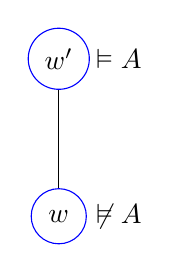
\begin{tikzpicture}
      \node [mstate] (1) at (0, 0) {$w'$};
      \node [right=10pt] at (1) {$\vDash A$};

      \node [mstate] (2) at (0, -2) {$w$};
      \node [right=10pt] at (2) {$\not\vDash A$};

      \draw (1) edge (2);
    \end{tikzpicture}
  \end{center}
\end{eg}

\begin{eg}
  This time consider the statement $w \vDash \neg \neg A \to A$. This takes some work to unravel.

  We need a world $w$ such that for all $w' \geq w$, if $w' \vDash \neg \neg A$, then $w' \vDash A$. If we unravel a bit more, we find that $w' \vDash \neg \neg A$ means for any $w'' \geq w'$, we can find some $w''' \geq w''$ such that $w''' \vDash A$.

  It is easy to see that actually in the model of the previous question, $w \not\vDash \neg \neg A \to A$, since $w \vDash \neg \neg A$, but $w \not\vDash A$.
\end{eg}

\begin{eg}
  The following model is a counter-model for $\neg \neg A \vee \neg A$:
  \begin{center}
    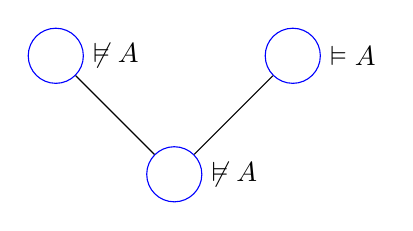
\begin{tikzpicture}
      \node [mstate] (b) at (0, 0) {};
      \node [right=10pt] at (b) {$\not\vDash A$};

      \node [mstate, above right=of b] (r) {};
      \node [right=10pt] at (r) {$\vDash A$};

      \node [mstate, above left=of b] (l) {};
      \node [right=10pt] at (l) {$\not\vDash A$};

      \draw (b) edge (r);
      \draw (b) edge (l);
    \end{tikzpicture}
  \end{center}
  where the bottom world believes in neither $\neg \neg A$ nor $\neg A$, since it sees worlds where $\neg A$ is true and also worlds where $A$ is true.
\end{eg}

Usually, we don't talk about a particular world believing in something. We talk about an entire structure of possible worlds believing something.
\begin{notation}
  If the root world of our model is $w$, then we write
  \[
    \vDash \varphi \Longleftrightarrow w \vDash \varphi.
  \]
\end{notation}
Almost by definition, if $\vDash \varphi$, then for any world $w'$, we have $w' \vDash \varphi$.

\begin{ex}
  Find a possible world model that does not believe Peirce's law.
\end{ex}

One can readily verify that classically, we have $(A \to B) \to B$ is equivalent to $A \vee B$, but they are not constructively equivalent.
\begin{ex}
  Find a possible world model that $\vDash (A \to B) \to B$, but does not $\vDash A \vee B$.
\end{ex}

\begin{ex}
  Find a possible world model that $\vDash (A \to B) \to B$ but does not believe $\vDash (B \to A) \to A$.
\end{ex}

\begin{ex}
  Find a possible world model that does not believe in $\vDash (A \to B) \vee (B \to A)$.
\end{ex}

Possible world semantics can be used for all sorts of logical systems, not just propositional logic. In general, the notion of accessibility need not be a partial order, but can be anything we want. Also, we do not necessarily have to require persistence. Of course, we also need to modify the according notion of a world.

\begin{eg}
  If we want to produce possible world semantics for constructive first-order logic, we need to modify our definition of worlds so that they have ``elements''. Assuming we have done so, we can encode $\forall$ and $\exists$ using the following rules:
  \begin{itemize}
    \item $w \vDash \exists x, F(x)$ if there is some $y \in w$ for which $w \vDash F(y)$.
    \item $w \vDash \forall x, F(x)$ if for all $w' \geq w$ and $x \in w'$, we have $w' \vDash F(x)$.
  \end{itemize}
  The second condition is much stronger than the naive ``for all $x \in w$, we have $w \vDash F(x)$'', because the $w'' \geq w$ may have many more elements. What our condition say is that $w$ somehow has a ``global'' way of showing that everything satisfies $F$.
\end{eg}

Let's talk a bit about persistence of formulae. We $\varphi$ is persistent iff $w \vDash\varphi$, $w' \geq w$ implies $w' \vDash \varphi$. By definition, all atomic formulae are persistent by stipulation. We can prove by induction that all formulae are persistent. This is just a massive yet easy proof by cases, and we will not do so.

\begin{eg}
  The proposition $A \to \neg \neg A$ is valid all possible world models.

  % To see this, we note that if we have a world $w$ that believes in $A$, then by persistence, any world that $A$ sees also believes in $A$. We want to show that it does not believe in $\neg A$. % complete proof, make use of reflexivity and transitivity
\end{eg}

% insert talk about finiteness of possible world models, therefore decidable.

Now suppose we have a possible world model in front of us. Then given a formula $\varphi$, the set of worlds that believe $\varphi$ is an upward-closed subset of the frame. So we can think of the truth value of $\varphi$ as these upward-closed set.
\begin{eg}
  Suppose we have the following worlds:
  \begin{center}
    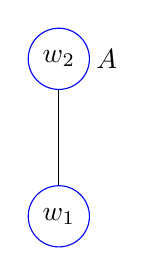
\begin{tikzpicture}
      \node [mstate] (1) at (0, 0) {$w_2$};
      \node [right=10pt] at (1) {$A$};

      \node [mstate] (2) at (0, -2) {$w_1$};

      \draw (1) edge (2);
    \end{tikzpicture}
  \end{center}
  So the top world only believes $A$, and the root world doesn't believe anything. The possible truth values are
  \[
    \emptyset, \{w_2\}, \{w_1, w_2\}.
  \]
  This is indeed the three-valued algebra we used to disprove Peirce's law. % check
\end{eg}
What can we say about the collection of upward-closed subset of frames, ie. our truth values? Under inclusion, it is easy to see that these are complete and co-complete, ie. we have all infinite unions and intersections.
\begin{defi}[Heyting algebra]\index{Heyting algebra}
  A Heyting algebra is a complete poset with joins $\wedge$ and $\vee$ and an operator $\to$ such that $A \Rightarrow B$ is the largest $C$ such that
  \[
    C \wedge A \leq B.
  \]
\end{defi}
We would expect
\[
  A \Rightarrow B = \vee \{C : C \wedge A \leq B\}.
\]
The only thing we need to check is that this choice of $A \Rightarrow B$ does indeed satisfy $(A \Rightarrow B) \wedge A \leq B$. % fix this!

The thought is that Heyting algebras would ``validate'' all constructive theses, by interpreting $\wedge$ with $\wedge$, $\vee$ with $\vee$ and $\rightarrow$ with $\Rightarrow$.

In other words, if we try to build a truth table for a formula with values in a Heyting algebra, we will get the top element $\top$ all the time iff the formula is constructively valid. So we have a parallel between the relation between classical logic and boolean algebras, and constructive logic and Heyting algebras.

Note that in classical logic, we only ever use the two-element boolean algebra. If we use the 4-element Boolean algebra, then we would detect the same set of tautologies. However, in the case of constructive logic we genuinely need all Heyting algebras.

\begin{lemma}
  Any formula with a natural deduction proof not using the rule for classical negation is true in all possible world models.
\end{lemma}
For any frame $F$, every such formula is satisfied by every possible world model on that frame. We say it is \emph{valid on $F$}. Such formulae are valid on all quasi-ordered sets with a bottom element.

\begin{proof}
  The hard case is implication. Suppose we have a natural deduction proof of $A \to B$. The last rule is a $\to$-introduction. So by the induction hypothesis, every world that believes $A$ also believes $B$. Now let $w$ be a world that believes all the other undischarged assumptions in $A \to B$. By persistence, every $w' \geq w$ believes similarly. So any $w' \geq w$ that believes $A$ also believes $B$. So $w \vDash A \to B$.
\end{proof}

\subsection{Negative interpretation}
Suppose a constructive logician found a classical logician, and then they try to talk to each other. Then they would find that they disagree on a lot of things. The classical logician has no problems accepting $\neg \neg A \to A$, but the constructive logician thinks that is nonsense. Can they make sense of each other?

The classical logician can understand the constructive logician via possible world semantics. He could think that when the constructive logician says a proposition is false, they mean there are possible world models where the proposition fails. This is all fine.

But can a constructive logician make sense of the classical logician? When the constructivist sees $A \vee B$, he thinks that either we can prove $A$, or we can prove $B$. However, the classical logician views this as a much weaker statement. It is more a long the lines of ``it is not true that $A$ and $B$ are both false''. In general, we can try to interpret classical statements by putting in enough negations:
\begin{center}
  \begin{tabular}{cc}
    \toprule
    Classical proposition & Constructive interpretation\\
    \midrule
    $A \vee B$ & $\neg (\neg A \vee \neg B)$\\
    $A \wedge B$& $A \wedge B$\\
    $\exists x\; W(x)$ & $\neg \forall x \neg W(x)$\\
    $A \to B$ & $\neg (A \wedge \neg B)$\\
    \bottomrule
  \end{tabular}
\end{center}
This gives rise to the \emph{negative interpretation} of classical logic into constructive logic, due to G\"odel:
\begin{defi}[Negative interpretation]\index{negative interpretation}
  Given a proposition $\phi$, the interpretation $\phi^*$ is defined recursively by
  \begin{itemize}
    \item $\bot^* = \bot$.
    \item If $\varphi$ is atomic, then $\varphi^* = \neg\neg \varphi$.
    \item If $\varphi$ is negatomic, then $\varphi^* = \varphi$.
    \item If $\varphi = \psi \wedge \theta$, then $\varphi^* = \psi^* \wedge \theta^*$.
    \item If $\varphi = \psi \vee \theta$, then $\varphi^* = \neg (\neg \psi^* \wedge \neg \theta^*)$.
    \item If $\varphi = \forall x\; \psi(x)$, then $(\forall x)(\psi^*(x))$.
    \item If $\varphi = \psi \to \theta$, then $\varphi^* = \neg(\psi^* \wedge \neg \theta^*)$.
    \item If $\varphi = \exists \; \psi(x)$, then $\varphi^* = \neg \forall x \neg \psi^*(x)$.
  \end{itemize}
\end{defi}
One can check that we always have $\vdash \varphi \to \varphi^*$. So the constructive version is always stronger.

\begin{defi}[Stable formula]\index{stable formula}
  A formula is \emph{stable} if
  \[
    \vdash \varphi^* \to \varphi.
  \]
\end{defi}

\begin{lemma}
  Any formula built up from negated and doubly negated atomics by $\neg$, $\wedge$ and $\forall$ is stable.
\end{lemma}

\begin{proof}
  By induction on formulae. The base case is immediate, using the fact that $\neg \neg \neg A \to \neg A$. More generally, we have
  \[
    (((p \to q) \to q) \to q) \to p \to q.
  \]
  It is less confusing to prove this in two steps, and we will write $\lambda$-terms for our proofs. First note that if we have $f: A \to B$, then we can obtain $f^T: (B \to q) \to A \to q$ for any $q$, using
  \[
    f^T = \lambda g_{B \to q}. \lambda a_A: g(f(a)).
  \]
  So it suffices to prove that
  \[
    p \to (p \to q) \to q,
  \]
  and the corresponding term is
  \[
    \lambda x_p. \lambda g_{p \to q}. g x
  \]
  We now proceed by induction.
  \begin{itemize}
    \item Now assume that we have proofs of $\neg \neg p \to p$ and $\neg \neg q \to q$. We want to prove $p \wedge q$ from $\neg \neg (p \wedge q)$. It suffices to prove $\neg \neg p$ and $\neg \neg q$ form $\neg \neg (p \wedge q)$, and we will just do the first one by symmetry.

      We suppose $\neg p$. Then we know $\neg (p \wedge q)$. But we know $\neg \neg (p \wedge q)$. So we obtain a contradiction. So we have proved that $\neg \neg p$.
    \item Note that we have
      \[
        \vdash \exists x \neg \neg \varphi(x) \to \neg \neg \exists x \varphi(x),
      \]
      but not the other way round. For universal quantification, we have
      \[
        \neg \neg \forall x \varphi(x) \to \forall x \neg \neg \varphi(x),
      \]
      but not the other way round. We can construct a proof as follows:
      \begin{prooftree}
        \AxiomC{$[\forall x) \varphi(x)]^1$}
        \elim{$\forall$}
        \UnaryInfC{$\varphi(a)$}
        \AxiomC{$[\neg \varphi(x)]^2$}
        \elim{$\to$}
        \BinaryInfC{$\to$}
        \intron{$\to$}{1}
        \UnaryInfC{$\neg \forall x \varphi(x)$}
        \AxiomC{$[\neg \neg \forall x \varphi(x)]^3$}
        \elim{$\to$}
        \BinaryInfC{$\bot$}
        \intron{$\to$}{2}
        \UnaryInfC{$\neg \neg \varphi(a)$}
        \intro{$\forall$}
        \UnaryInfC{$\neg \neg \forall \varphi(x)$}
        \intron{$\to$}{3}
        \UnaryInfC{$\neg \neg \forall x F(x) \to \forall x \neg \neg F(x)$}
      \end{prooftree}
      We now want to show that if $\varphi$ is stable, then $\forall x \varphi(x)$ is stable. In other words, we want
      \[
        \neg \neg \forall x \varphi^*(x) \to \forall x \varphi^*(x).
      \]
      But form $\neg \neg \forall x \varphi^*(x)$, we can deduce $\forall x \neg \neg \varphi^*(x)$, which implies $\forall x \varphi^* (x)$.
  \end{itemize}
  So every formula in the range of the negative interpretation is stable. Every stable formula is equivalent to its double negation (classically). Every formula is classically equivalent to a stable formula.
\end{proof}
So if a constructive logician meets a classical logician who is making some bizarre assertions about first order logic. To make sense of this, the constructive logician can translate it to its negative interpretation, which the classical logician thinks is equivalent to the original one. And now these interpretations follow the law of excluded middle.

\subsection{Constructive mathematics}
We now want to try to do mathematics constructively. We note that even classically, if we do not have the law of excluded middle, then we have many distinct notions of ``finite set''. When we go constructive, things get more complicated.

We look at several possible definitions of finite sets.
\begin{defi}[Kuratowski finite]\index{Kuratowski finite}\index{finite!Kuratowski}
  We define ``finite'' recursively: $\emptyset$ is Kuratowski finite. If $x$ is Kuratowski finite, then so is $x \cup \{y\}$.
\end{defi}

There is a separate definition of $N$-finiteness:
\begin{defi}[$N$-finite]\index{$N$-finite}\index{finite!$N$}
  $\emptyset$ is $N$-finite. If $x$ is $N$-finite, and $y \not \in x$, then $x \cup \{y\}$ is $N$-finite.
\end{defi}
These two definitions are not the same! In a $N$-finite set, we know any two things are either equal, or they are not, as this is built into the definition of an $N$-finite set. However, in the case of Kuratowski finite, this is not true, since we don't have the law of excluded middle. We say $N$-finite sets have \term{decidable equality}.
If we want to do constructive arithmetic, the correct notion is $N$-finiteness.

We can still define natural numbers as the smallest set containing $\emptyset$ and is closed under successor. This gives us $N$-finite sets, but the least number principle is dodgy. It turns out the least number principle implies excluded middle.

It is helpful to note the following two definitions:
\begin{defi}[Non-empty set]\index{non-empty set}
  A set $x$ is non-empty if $\neg (\forall y)(y \not \in x)$.
\end{defi}

\begin{defi}[Inhabited set]\index{inhabited set}
  A set $x$ is inhabited if $(\exists y)(y \in x)$.
\end{defi}

\section{Model theory}

\subsection{Universal theories}
Recall the following definition:
\begin{defi}[Universal theory]\index{universal theory}
  A universal theory is a theory that can be axiomatized in a way such that all axioms are of the form
  \[
    (\forall \cdots)(\text{stuff not involving quantifiers})\tag{$*$}
  \]
\end{defi}
For example, groups, rings, modules etc. are universal theories. It is easy to see that if we have a model of a universal theory, then any substructure is also a model.

It turns out the converse is also true! If a theory is such that every substructure of a model is a model, then it is universal. This is a very nice result, because it gives us a correspondence between syntax and semantics.

The proof isn't very hard, and this is the first result we will prove about model theory. We begin with some convenient definitions.
\begin{defi}[Diagram]\index{diagram}
  Let $\mathcal{L}$ be a language and $\mathcal{M}$ a structure of this language. The \emph{diagram} of $\mathcal{M}$ is the theory obtained by adding a constant symbol $a_x$ for each $x \in \mathcal{M}$, and then taking the axioms to be all quantifier-free sentences that are true in $M$. We will write the diagram as $D(\mathcal{M})$.
%
% The \emph{diagram} of a structure $\mathcal{M}$ is the theory obtained by expanding $\mathcal{M}$ by giving names to all its elements, and then recording all atomic truths about them.
\end{defi}
%
%\begin{defi}[Expansion and reduct of structure]\index{expansion of structure}\index{reduct of structure}
% The \emph{expansion} of a structure is what we get when we add more gadgets, ie. add more things to the signature. A \emph{reduct} of a structure is what we get when we forget gadgets.
%\end{defi}
%Here we change the signature but not the carrier set.
%
%\begin{eg}
% $\bra \Q, 0, +, \leq\ket$ is an expansion of $\bra \Q, \leq\ket$. Conversely, $\bra \Q, \leq\ket$ is a reduct of $\bra \Q, 0, +, \leq \ket$.
%\end{eg}
%
%\begin{defi}[Extension and substructure]\index{extension}\index{substructure}
% An \emph{extension} of a structure is a superstructure of the same signature. A substructure is what you think it is.
%\end{defi}
%
%\begin{eg}
% $\bra \R, \leq\ket$ is an extension of $\bra \Q, \leq\ket$, and $\bra \Q, \leq\ket$ is a substructure of $\bra \R, \leq\ket$.
%\end{eg}

\begin{lemma}
  Let $T$ be a consistent theory, and let $T_{\forall}$ be the set of all universal consequences of $T$, ie. all things provable from $T$ that are of the form $(*)$. Let $\mathcal{M}$ be a model of $T_\forall$. Then $T \cup D(\mathcal{M})$ is also consistent.
\end{lemma}

\begin{proof}
  Suppose $T \cup D(\mathcal{M})$ is not consistent. Then there is an inconsistency that can be derived from finitely many of the new axioms. Call this finite conjunction $\psi$. Then we have a proof of $\neg \psi$ from $T$. But $T$ knows nothing about the constants we added to $T$. So we know $T\vdash \forall \mathbf{x} \neg \psi$. This is a universal consequence of $T$ that $\mathcal{M}$ does not satisfy, and this is a contradiction.
\end{proof}

\begin{thm}
  A theory $T$ is universal if and only if every substructure of a model of $T$ is a model of $T$.
\end{thm}

\begin{proof}
  $\Rightarrow$ is easy. For $\Rightarrow$, suppose $T$ is a theory such that every substructure of a model of $T$ is still a model of $T$.

  Let $\mathcal{M}$ be an arbitrary model of $T_\forall$. Then $T \cup D(\mathcal{M})$ is consistent. So it must have a model, say $\mathcal{M}^*$, and this is in particular a model of $T$. Moreover, $\mathcal{M}$ is a submodel of $\mathcal{M}^*$. So $\mathcal{M}$ is a model of $T$.

  So any model of $T_{\forall}$ is also a model of $T$, and the converse is clearly true. So we know $T_{\forall}$ is equivalent to $T$.
\end{proof}

\subsection{Products}
In model theory, we would often like to produce new models of a theory from old ones. One way to do so is via products.

We will use $\lambda$-notation to denote functions.
\begin{defi}[Product of structures]\index{product of structures}
  Suppose $\{A_i\}_{i \in I}$ is a family of structures of the same signature. Then the product
  \[
    \prod_{i \in I} A_i
  \]
  has carrier set the set of all functions
  \[
    \alpha: I \to \bigcup_{i \in I} A_i
  \]
  such that $\alpha(i) \in A_i$.

  Given an $n$-ary function $f$ in the language, the interpretation in the product is given pointwise by
  \[
    f(\alpha_1, \cdots, \alpha_n) = \lambda i. f(\alpha_1(i), \cdots, \alpha_n(i)).
  \]
  Relations are defined by
  \[
    \varphi(\alpha_1, \cdots, \alpha_n) = \bigwedge_{i \in I} \varphi(\alpha_1(i), \cdots, \alpha_n(i)).
  \]
\end{defi}
The natural question to ask is if we have a model of a theory, then is the product a model again? We know this is not always true. For example, the product of groups is a group, but the product of total orders is not a total order.

We say a product \emph{preserves} a formula $\varphi$ if
\[
  \prod_{i \in I} A_i \vDash \varphi \Longleftrightarrow \forall_{i \in I}, A_i \vDash \varphi
\]
What sort of things do products preserve? As we know from undergraduate mathematics, theories such as groups and rings are preserved.
\begin{defi}[Equational theory]\index{equational theory}
  An equational theory is a theory all of whose axioms are of the form
  \[
    (\forall \mathbf{x}) (w_1(\mathbf{\mathbf{x}}) = w_2(\mathbf{x})),
  \]
  where $w_i$ are some terms in $\mathbf{x}$.
\end{defi}
It is not hard to see that models of equational theories are preserved under products.

It turns out actually the class of things preserved by products is much more general.

\begin{defi}[Horn clause]\index{Horn clause}
  A \emph{Horn clause} is a disjunction of atomics and negatomics of which at most one disjunct is atomic. % need a definition of negatomic somewhere

  It is usually better to think of Horn clauses as formulae of the form
  \[
    \left(\bigwedge \varphi_i\right) \to \chi
  \]
  where $\varphi_i$ and $\chi$ are atomic formulae. Note that $\bot$ is considered an atomic formula.

  A \term{universal Horn clause}\index{Horn clause!universal} is a universal quantifier followed by a Horn clause.
\end{defi}

\begin{eg}
  Transitivity, symmetry, antisymmetry, reflexivity are all universal Horn clauses.
\end{eg}

\begin{prop}
  Products preserve (universal) Horn formulae.
\end{prop}

\begin{proof}
  Suppose every factor
  \[
    A_i \vDash (\forall \mathbf{x}) \bigwedge \varphi_i(\mathbf{x}) \to \chi(\mathbf{x}).
  \]
  We want to show that the product believes in the same statement. So let $(f_1, \cdots, f_k)$ be a tuple in the product of the right length satisfying the antecedent, ie. for each $n \in I$, we have
  \[
    A_n \vDash \varphi_i (f_1(n), \cdots, f_k(n))
  \]
  for each $i$, But then by assumption,
  \[
    A_n \vDash \chi(f_1(n), \cdots, f_k(n))
  \]
  for all $n$. So the product also believes in $\varphi_j(f_1, \cdots, f_n)$. So we are done.
\end{proof}

\subsubsection*{Reduced products}
Unfortunately, it is rarely the case that products give us new interesting models. However, \emph{reduced} products do.

Reduced products arise from having a filter on the index set.
\begin{defi}[Filter]\index{filter}
  Let $I$ be a set. A \emph{filter} on $I$ is a (non-empty) subset $F \subseteq P(I)$ such that $F$ is closed under intersection and superset. A \term{proper filter}\index{proper filter}\index{filter!proper} is a filter $F \not= P(I)$.
\end{defi}

The intuition to hang on to is that $F$ captures the intuition of ``largeness''.
\begin{eg}
  Take $I = \N$, and $F$ the set of cofinite subsets of $\N$, namely the sets whose complement are finite, then $F$ is a filter.

  Similarly, we can take $F$ to contain the set of naturals with asymptotic density $1$.
\end{eg}

\begin{eg}
  Let
  \[
    F = \{x \subseteq \N: 17 \in \N\}
  \]
  Then this is a \emph{maximal} proper filter.
\end{eg}
This is a rather silly filter. We will see later that model-theoretically, these give us uninteresting reduced products.

\begin{defi}[Principal filter]\index{principal filter}
  A \emph{principal filter} is a filter of the form
  \[
    F = \{X \subseteq I: x \not\in X\}
  \]
  for some $x \in I$.
\end{defi}
We don't tend to care about principal filter, as they are boring.

\begin{defi}[Complete filter]\index{complete filter}\index{$\kappa$-complete filter}\index{filter!complete}\index{filter!$\kappa$-complete}
  A filter $F$ is $\kappa$-complete if it is closed under intersection of $<\kappa$ many things.
\end{defi}

\begin{eg}
  By definition, every filter is $\aleph_0$-complete.
\end{eg}

\begin{eg}
  Principal filters are $\kappa$-complete for all $\kappa$.
\end{eg}

A natural question is, are there any non-principal ultrafilters that are $\aleph_1$ complete? It turns out this is a deep question, and a lot of the study of set theory originated from this question.

Filters on $I$ form a complete poset under inclusion, with top element given by $F = P(I)$. Moreover, the \emph{proper} filters are a chain complete poset. Thus, by Zorn's lemma, there are \emph{maximal} proper filters.
\begin{defi}[Ultrafilter]\index{ultrafilter}
  An \emph{ultrafilter} is a maximal filter.
\end{defi}

We saw that principal filters are ultra. Are there non-principal ultrafilters? Fortunately, by Zorn's lemma, they do exist.
\begin{eg}
  By Zorn's lemma, there is a maximal filter extending the cofinite filter on $\N$, and this is non-principal.
\end{eg}
It turns out it is impossible to explicitly construct a non-principal ultrafilter, but Zorn's lemma says they exist.

%The dual notion to filter is an \term{ideal}, which are closed under union and subsets. They are called ideals because they are ideals in the corresponding boolean ring.

Now we can get to reduced products.
\begin{defi}[Reduced product]\index{reduced product}\index{product!reduced}
  let $\{A_i: i \in I\}$ be a family of structures, and $F$ a filter on $I$. We define the \emph{reduced product}
  \[
    \prod_{i \in I} A_i / F
  \]
  as follows: the underlying set is the usual product $\prod A_i$ quotiented by the equivalence relation
  \[
    \alpha \sim_F \beta \Longleftrightarrow \{i : \alpha(i) = \beta(i)\} \in F
  \]
  Given a function symbol $f$, the interpretation of $f$ in the reduced product is induced by that on the product.

  Given a relational symbol $\varphi$, we define
  \[
    \varphi(\alpha_1, \cdots, \alpha_n) \Longleftrightarrow \{i : \varphi(\alpha_1(i), \cdots, \alpha_n(i))\} \in F.
  \]
  If $F$ is an ultrafilter, then we call it the \term{ultraproduct}. If all the factors in an ultraproduct are the same, then we call it an \term{ultrapower}.
\end{defi}
It is an easy exercise to show that these are all well-defined. If we view the filter as telling us which subsets of $I$ are ``large'' then, our definition of reduced product says we regard two functions in the reduced products as equivalent if they agree on a ``large'' set.

Note that if our filter is principal, say $F = \{J \subseteq I: i \in J\}$, then the reduced product is just isomorphic to $A_i$ itself. So this is completely uninteresting.

%Suppose we have a family $\{A_i: i \in I\}$ of structures. We can as usual form the product $\prod A_i$. Suppose $F$ is a filter. Recall that $F$ is supposed to capture the notion of largeness. So we now form an equivalence relation on the elements by saying two elements are equal if they agree on a large set: For $f, g \in \prod A_i$, we say
%
%Observe that the definition of ``filter'' is designed to make $\sim_F$ an equivalence relation.
%
%\begin{defi}[Congruence relation]\index{congruence relation}
% We say an equivalence relation $\sim$ on $X$ is a \emph{congruence relation} for a function $f: X^m \to X$ iff for all $\mathbf{x}, \mathbf{y} \in X^m$ such that $x_i \sim y_i$ for all $i$, then
% \[
% f(\mathbf{x}) \sim f(\mathbf{y}).
% \]
%\end{defi}
%This in some sense says $f$ cannot tell equivalent things apart. Alternatively, this says $f$ passes on to a function $X^m/\sim \to X/\sim$.
%
%We can similarly define the notion of being a congruence relation for a predicate.
%\begin{eg}
% Equivalence mod $p$ is a congruence relation for $+$ and $\times$, but not for exponentiation.
%\end{eg}
%
%We now consider the quotient
%\[
% \prod_{i \in I} A_i/\sim_{F} = \prod_{i \in I} A_i /F.
%\]
%It is a very important, and also trivial, fact, that $\sim_F$ is a congruence relation for all the operations on the $A_i$ that are inherited by the product. The result is called the \term{reduced product} modulo $F$.

Reduced products preserve various things, but not everything. For example, the property of being a total order is in general not preserved by reduced products. So we still have the same problem.

But if the filter $F$ is an \emph{ultrafilter}, then nice things happen.

\begin{thm}[\L{}o\'s theorem]\index{\L{}o\'s theorem}
  Let $\{A_i: i \in I\}$ be a family of structures of the same (first-order) signature, and $\mathcal{U} \subseteq P(I)$ an ultrafilter. Then
  \[
    \prod_{i \in I} A_i/\mathcal{U} \vDash \varphi \Longleftrightarrow \{i: A_i \vDash \varphi\} \in \mathcal{U}.
  \]
  In particular, if $A_i$ are all models of some theory, then so is $\prod A_i / \mathcal{U}$.
\end{thm}

The key of the proof is the following lemma, which is a nice exercise:
\begin{lemma}
  Let $F$ be a filter on $I$. Then the following are equivalent:
  \begin{enumerate}
    \item $F$ is an ultrafilter.
    \item For $X \subseteq I$, either $X \in F$ or $I\setminus X \in F$ (``$F$ is prime'').
    \item If $X, Y \subseteq I$ and $X \cup Y \in I$, then $X \in I$ or $Y \in I$.
  \end{enumerate}
\end{lemma}
With this in mind, it is hard not to prove the theorem.

% How should we think about the elements of the ultraproduct? One can certainly view its elements as equivalence classes of elements in the product. However, sometimes it is helpful to think of the carrier set as the product itself, and instead weaken to notion of equality to say two things are equal if the are equivalent under $\sim_\mathcal{U}$.

%Note that there is an elementary embedding $K: \mathcal{M} \to \mathcal{M}^I/\mathcal{U}$ given by sending $m \in \mathcal{M}$ to $[\lambda i. m] \in \mathcal{M}^I/\mathcal{U}$.

%This is the natural inclusion one can think of, and we can show this is in fact elementary. It suffices to show that for any $m \in \mathcal{M}$, if there an $x \in \mathcal{M}^I/\mathcal{U}$ such that
%\[
% \mathcal{M}^I/\mathcal{U} \vDash \varphi(x, \iota(m)),
%\]
%then there is such an $x$ that is in the image of $\iota$.
%
%Consider such an $x$. It is an equivalence class of a family of functions which is almost everywhere related to $m$ by $\varphi$. So by \L{}o\'s theorem, tthere must be some $x' \in \mathcal{M}$ such that
%\[
% \mathcal{M} \vDash \varphi(x, m).
%\]
%Then we have
%\[
% \mathcal{M}^I/\mathcal{U} \vDash \varphi(\iota(x'), \iota(m')).
%\]
Let's now look at some applications of \L{}o\'s theorem.

Recall the compactness theorem of first order logic --- if we have a theory $T$ such that every finite subset of $T$ has a model, then so does $T$. The way we proved it was rather roundabout. We proved the completeness theorem of first order logic. Then we notice that if every finite subset of $T$ has a model, then every finite subset of $T$ is consistent. Since proofs are finite, we know $T$ is consistent. So by completeness, $T$ has a model.

Now that we are equipped with ultraproducts, it is possible to prove the compactness theorem directly!
\begin{thm}[Compactness theorem]\index{compactness theorem}
  Let $T$ be a theory in first order logic such that every finite subset has a model. Then $T$ has a model.
\end{thm}

\begin{proof}
  Let $\Delta$ be such a theory. Let $S = \mathcal{P}_{\aleph_0}(\Delta)$ be the set of all finite subsets of $\Delta$. For each $s \in S$, we pick a model $\mathcal{M}_s$ of $s$.

  Given $s \in S$, we define
  \[
    X_s = \{t \in S: s \subseteq t\}.
  \]
  We notice that $\{X_s: s \in S\}$ generate a proper filter on $S$. We extend this to ultrafilter $\mathcal{U}$ by Zorn's lemma. Then we claim that
  \[
    \prod_{s \in S} \mathcal{M}_s/\mathcal{U}\vDash \Delta.
  \]
  Indeed, for any $\varphi \in \Delta$, we have
% To see this, we note that for any $\varphi \in \Delta$, we have $X_{\{\varphi\}} \in \mathcal{U}$. Also, for any $s \in X_{\{\varphi\}}$, we have $\mathcal{M}_s \vDash \varphi$. So
  \[
    \{s: \mathcal{M}_s \vDash \varphi\} \supseteq X_{\{\varphi\}} \in \mathcal{U}.
  \]
\end{proof}

\begin{eg}
  Let $T$ be the theory consisting of all first-order statements true in $\bra \R, 0, 1, +, \times\ket$. Add to $T$ a constant $\varepsilon$ and the axioms $\varepsilon < \frac{1}{n}$ for all $n \in \N$. Then for any finite subset of this new theory, $\R$ is still a model, by picking $\varepsilon$ small enough. So by the compactness theorem, we know this is consistent.

  Using \emph{our} proof of the compactness theorem, we now have a ``concrete'' model of real numbers with infinitesimals --- we just take the ultraproduct of infinitely many copies of $\R$.
\end{eg}

\subsection{Ehrenfeucht--Mostowski theorem}
\begin{defi}[Skolem function]\index{Skolem function}
  \emph{Skolem functions} for a structure are functions $f_\varphi$ for each $\varphi \in \mathcal{L}$ such that if
  \[
    \mathcal{M} \vDash \forall \mathbf{x} \exists \mathbf{y} \varphi(\mathbf{x}, \mathbf{y}),
  \]
  then
  \[
    \mathcal{M} \vDash \forall \mathbf{x} \varphi(\mathbf{x}, f_\varphi(\mathbf{x})).
  \]
\end{defi}

\begin{defi}[Skolem hull]\index{Skolem hull}
  The \emph{Skolem hull} of a structure is obtained from the constants term by closure under the Skolem functions.
\end{defi}

\begin{defi}[Elementary embedding]\index{elementary embedding}
  Let $\Gamma$ be a set of formulae. A function $i: \mathcal{M}_1 \to \mathcal{M}_2$ is \term{$\Gamma$-elementary} iff for all $\varphi \in \Gamma$ we have $\mathcal{M}_1 \vDash \varphi(\mathbf{x})$ implies $\mathcal{M}_2 \vDash \varphi(i(\mathbf{x}))$.

  If $\Gamma$ is the set of all formulae in the language, then we just say it is \emph{elementary}.
\end{defi} % move this to earlier
Usually, we take $\Gamma$ to be the set of all formulae, and $\mathcal{M}_1$ to be a substructure of $\mathcal{M}_2$.

\begin{eg}
  It is, at least intuitively, clear that the inclusion $\bra \Q, \leq\ket \hookrightarrow \bra \R, \leq \ket$ is elementary.

  However, $\Q$ as a field is \emph{not} elementary as a substructure of $\R$ as a field.
\end{eg}

Note that first order logic is not decidable. However, \emph{monadic} first order logic is.
\begin{defi}[Monadic first order logic]\index{monadic first order logic}\index{first order logic!monadic}
  \emph{Monadic first-order logic} is first order logic with only one-place predicates, no equality and no function symbols.
\end{defi}

\begin{prop}
  Monadic first-order logic is decidable.
\end{prop}

\begin{proof}
  Consider any formula $\varphi$. Suppose it involves the one-place predicates $p_1, \dots, p_n$. Given any structure $\mathcal{M}$, we consider the quotient of $\mathcal{M}$ by
  \[
    x \sim y \Leftrightarrow p_i (x) = p_i(y) \text{ for all i}.
  \]
  Then there are at most $2^n$ things in the quotient.

  Then given any transversal of the quotient, we only have to check if the formula holds for this transversal, and this is finite. So we can decide.
\end{proof}

\begin{defi}[Set of indiscernibles]\index{set of indiscernibles}
  We say $\bra I, \leq_I\ket$ is a \emph{set of indiscernibles} for $\mathcal{L}$ and a structure $\mathcal{M}$ with $I \subseteq \mathcal{M}$ if $\forall \varphi \in \mathcal{L}(M)$, with $\varphi$ of arity $n$, and for all increasing tuples $\mathbf{x}, \mathbf{y} \in I$,
  \[
    \mathcal{M} \vDash \varphi(\mathbf{x}) \Longleftrightarrow \mathcal{M} \vDash \varphi(\mathbf{y})
  \]
\end{defi}
This is weaker than just saying everything in there are the same.

\begin{eg}
  $\bra \Q, I\ket$ is a set of indiscernibles for $\bra \R, \leq\ket$.
\end{eg}

Let $T$ be a theory with infinite models. The general line of thought is --- can we get a model of $T$ with special properties?

Given any set $\mathcal{M}$, invent names for every member of $\mathcal{M}$. Add these names to the language of $T$. We add axioms to say all these constants are distinct. Since $T$ has infinite models, we know this theory has a model.

Let $\Omega$ be the set of countable ordinals, consider the language of $\R$, and add a name to this language for every countable ordinal. We further add axioms to say that $\alpha < \beta$ in the ordering of $\R$ whenever $\alpha < \beta$ as ordinals.

Again by compactness, we find that this has a model. So we can embed the set of countable ordinals into a model of reals, which we know is impossible for the genuine $\R$. However, in general, there is no reason to believe these elements are a set of indiscernibles. What Ehrenfeucht--Mostowski says is that we can in fact do so.

\begin{thm}[Ehrenfeucht--Mostowski theorem (1956)]\index{Ehrenfeucht--Mostowski theorem}
  Let $\bra I, \leq\ket$ be a total order, and let $T$ be a theory with infinite models. Suppose we have a unary predicate $P$ and a $2$-ary relation $\preccurlyeq \in \mathcal{L}(T)$ such that
  \[
    T \vdash \text{$\preccurlyeq$ is a total order on $\{x: P(x)\}$}.
  \]
  Then $T$ has a model $\mathcal{M}$ with a copy of $I$ as a sub-order of $\preccurlyeq$, and the copy of $I$ is a set of indiscernibles. Moreover, we can pick $\mathcal{M}$ such that every order-automorphism of $\bra I, \leq \ket$ extends to an automorphism of $\mathcal{M}$.
\end{thm}

We will give two proofs of this result. We first give the original proof of Ehrenfeucht--Mostowski, which uses Ramsey theory.
\begin{proof}
  Let $T$ and $\bra I, \leq \ket$ be as in the statement of the theorem. We add to $\mathcal{L}(T)$ names for every element of $I$, say $\{c_i: i \in I\}$. We add axioms that says $P(c_i)$ and $c_i \preccurlyeq c_j$ whenever $i < j$. We will thereby confuse the orders $\leq$ and $\preccurlyeq$, partly because $\leq$ is much easier to type. We call this theory $T^*$.

  Now we add to $T^*$ new axioms to say that the $c_i$ form a set of indiscernibles. So we are adding axioms like
  \[
    \varphi(c_i, c_j) \Leftrightarrow \varphi(c_{i'}, c_{j'})\tag{$*$}
  \]
  for all $i < j$ and $i' < j'$. We do this simultaneously for all $\varphi \in \mathcal{L}(T)$ and all tuples of the appropriate length. We call this theory $T^I$, and it will say that $\bra I, \leq\ket$ forms a set of indiscernibles. The next stage is, of course, to prove that $T^I$ is consistent.

  Consider any finite fragment $T'$ of $T^I$. We want to show that $T'$ is consistent. By finiteness, $T'$ only mentions finitely many constants, say $c_1 < \cdots < c_K$, and only involve finitely many axioms of the form $(*)$. Denote those predicates as $\varphi_1, \cdots, \varphi_n$. We let $N$ be the supremum of the arities of the $\varphi_i$.

  Pick an infinite model $\mathcal{M}$ of $T$. We write
  \[
    \mathcal{M}^{[N]} = \{A \subseteq \mathcal{M}: |A| = N\},
  \]
  For each $\varphi_i$, we partition $\mathcal{M}^{[N]}$ as follows --- given any collection $\{a_k\}_{k = 1}^N$, we use the order relation $\preccurlyeq$ to order them, so we suppose $a_k \preccurlyeq a_{k + 1}$. If $\varphi_i$ has arity $m \leq N$, then we can check whether $\varphi_i(a_1, \cdots, a_m)$ holds, and the truth value gives us a partition of $\mathcal{M}^{[N]}$ into 2 bits.

  If we do this for all $\varphi_i$, then we have finitely partitioned $\mathcal{M}^{[N]}$. By Ramsey's theorem, this has an infinite monochromatic subset, ie. a subset such that any two collection of $N$ members fall in the same partition. We pick elements $c_1, \cdots, c_K, \cdots, c_{K + N}$, in increasing order (under $\preccurlyeq$). We claim that picking the $c_1, \cdots, c_K$ to be our constants satisfy the axioms of $T'$.

  Indeed, given any $\varphi_i$ mentioned in $T'$ with arity $m < N$, and sequences $c_{\ell_1} < \cdots < c_{\ell_m}$ and $c_{\ell_1'} < \cdots < c_{\ell_m'}$, we can extend these sequences on the right by adding more of those $c_i$. Then by our choice of the colouring, we know
  \[
    \varphi_i(c_{\ell_1}, \cdots, c_{\ell_m}) \Leftrightarrow \varphi_i(c_{\ell_1'}, \cdots, _{\ell_m'}).
  \]
  So we know $T'$ is consistent. So $T^I$ is consistent. So we can just take a model of $T^I$, and the Skolem hull of the indiscernibles is the model desired.
\end{proof}

There is another proof of Ehrenfeucht--Mostowski due to Gaifman, using ultraproducts. We will sketch the proof here.

To do so, we need the notion of colimits.
\begin{defi}[Colimit]\index{colimit}
  Let $\{A_i: i \in I\}$ be a family of structures index by a poset $\bra I, \leq\ket$, with a family of (structure-preserving) maps $\{\sigma_{ij}: A_i \hookrightarrow A_j \mid i \leq j\}$ such that whenever $i \leq j \leq k$, we have
  \[
    \sigma_{jk} \sigma_{ij} = \sigma_{ik}.
  \]
  In particular $\sigma_{ii}$ is the identity. A \emph{colimit} or \term{direct limit} of this family of structures is a ``minimal'' structure $A_\infty$ with maps $\sigma_i: A_i \hookrightarrow A_\infty$ such that whenever $i \leq j$, then the maps
  \[
    \begin{tikzcd}
      A_i \ar[d, "\sigma_{ij}"'] \ar[r, "\sigma_i"] & A_\infty\\
      A_j \ar[ur, "\sigma_j"']
    \end{tikzcd}
  \]
  commute.

  By ``minimal'', we mean if $A_\infty'$ is another structure with this property, then there is a unique inclusion map $A_\infty \hookrightarrow A_\infty'$ such that for any $i \in I$, the maps
  \[
    \begin{tikzcd}
      A_i \ar[r, "\sigma_i"] \ar[rd, "\sigma_i'"'] & A_\infty\ar[d, hook]\\
      & A_\infty'
    \end{tikzcd}
  \]
\end{defi}

\begin{eg}
  The colimit of a family of sets is obtained by taking the union of all of them, and then identifying $x \sim \sigma_{ij}(x)$ for all $x \in A_i$ and $i \leq j$.
\end{eg}

The key observation is the following:
\begin{significant}
  Every structure is a direct limit of its finitely generated substructures, with the maps given by inclusion.
\end{significant}
We will neither prove this nor make this more precise, but it will be true for the different kinds of structures we are interested in. In particular, for a poset, a finitely generated substructure is just a finite suborder, because there are no function symbols to ``generate'' anything in the language of posets.

To prove Ehrenfeucht--Mostowski, we construct a model satisfying the statement of Ehrenfeucht--Mostowski as the direct limit of structures indexed by finite subset of $I$:
\[
  \{\mathcal{M}_s: s \in \mathcal{P}(I)\}
\]
and when $s \subseteq t \in \mathcal{P}(I)$, we have an elementary embedding $\mathcal{M}_s \hookrightarrow \mathcal{M}_t$. We then note that if all the $\sigma_{ij}$ are elementary, then the $\sigma_i: A_i \hookrightarrow A_\infty$ are also elementary. In particular, if each $\mathcal{M}_s$ are models of our theory, then so is $A_\infty$.

We start by picking any infinite model $\mathcal{M}$ of $I$. By standard compactness arguments, we may wlog there is no last $\preccurlyeq$-thing in $\mathcal{M}$, and also that $J = \{x: P(x)\}$ is infinite. We pick $\mathcal{U}$ an ultrafilter on $J$ that contains all terminal segments of $\preccurlyeq$. Since $J$ does not have a last element, this is a non-principal ultrafulter.

We now write
\[
  L(\mathcal{M}) = \mathcal{M}^{|J|}/\mathcal{U}.
\]
We will define
\[
  \mathcal{M}_s = L^{|s|}(\mathcal{M}).
\]
In particular, $\mathcal{M}_{\emptyset} = \mathcal{M}$.

To construct the embedding, we consider the following two classes of maps:
\begin{enumerate}
  \item For any structure $\mathcal{M}$, there is a map $K = K(\mathcal{M}): \mathcal{M} \to L(\mathcal{M})$ given by the constant embedding.
  \item If $i$ is an embedding from $\mathcal{M}$ into $\mathcal{N}$, then there is an embedding
    \[
      L(i): L(\mathcal{M}) \to L(\mathcal{N}).
    \]
    which is ``compose with $i$ on the right''.
\end{enumerate}
It is easy to see that both of these maps are elementary embeddings, where we require $i$ to be elementary in the second case. Moreover, these maps are compatible in the sense that the following diagram always commutes:
\[
  \begin{tikzcd}
    \mathcal{M} \ar[r, "i"] \ar[d, "K(\mathcal{M})"] & \mathcal{N} \ar[d, "K(\mathcal{N})"]\\
    L(\mathcal{M}) \ar[r, "L(i)"'] & L(\mathcal{N})
  \end{tikzcd}
\]
%How do we construct these $\mathcal{M}_s$? We start with any model $\mathcal{M}$ of $T$. We are going to assume that there is no last $\preccurlyeq$-thing in $\mathcal{M}$, and also that the graph of $\preccurlyeq$ is infinite. We let $\mathcal{U}$ be a non-principal ultrafilter $J = \{x: P(x)\}$. Then we pick $\mathcal{M}_s$ to be the result of doing an ultrapower construction using $\mathcal{U}$, $|s|$ many times to $\mathcal{M}$. The tricky bit is to construct the embeddings.
%We define this by recursion. We write $\last(s)$ for the last element of $s$, and $\butlast(s)$ for $s \setminus \{\last(s)\}$. Given a structure $\mathcal{M}$, we write
%\[
%  L(\mathcal{M}) = \mathcal{M}^p/\mathcal{U}.
%\]
%We need two gadgets
%\begin{enumerate}
%  \item An elementary embedding $K(\mathcal{M}): \mathcal{M} \to L(\mathcal{M})$.
%  \item If $i$ is an embedding from $\mathcal{M}$ into $\mathcal{N}$, then there is an
%    \[
%      L(i): L(\mathcal{M}) \to L(\mathcal{N}).
%    \]
%    which is ``compose with $i$ on the right''.
%\end{enumerate}
%Moreover, these are compatible in the sense
%\[
%  \begin{tikzcd}
%    \mathcal{M} \ar[r, "i"] \ar[d, "K(\mathcal{M})"] & \mathcal{N} \ar[d, "K(\mathcal{N})"]\\
%    L(\mathcal{M}) \ar[r, "L(i)"] & L(\mathcal{N})
%  \end{tikzcd}
%\]
%We can now recursively define $I(s, t): \mathcal{M}_s \to \mathcal{M}_t$.
We now further consider the functions $\head$ and $\tail$ defined on finite linear orders by
\begin{align*}
  \head(a_1 < \cdots < a_n) &= a_1\\
  \tail(a_1 < \cdots < a_n) &= a_2 < \cdots < a_n.
\end{align*}
We can now define the embeddings recursively. We write $I(s, t)$ for the desired inclusion from $\mathcal{M}_s$ into $\mathcal{M}_t$.  We set
\begin{itemize}
  \item If $s = t$, then $I(s, t)$ is the identity.
  \item If $\head(s) = \head(t)$, then $I(s, t)$ is $L(I(\tail(s), \tail(t)))$.
  \item Otherwise, $I(s, t)$ is $K \circ I(s, \tail(t))$.
%  \item If $s = t$, then $I(s, t)$ is the identity.
%  \item If $\last(s) = \last(t)$, then $I(s, t)$ is $L(I(\butlast(s), \butlast(t)))$. Otherwise, it is $K \circ I(s, \butlast(t))$.
\end{itemize}
By our previous remark, we know these are all elementary embeddings, and that these maps form a commuting set. Thus, we obtain a direct limit $\mathcal{M}_\infty$.

Now we want to produce a copy of $I$ in the direct limit. So we want to produce a copy of $s$ in $\mathcal{M}_s$ for each $s$, such that the maps preserve these copies. It suffices to be able to do it in the case $|s| = 2$, and then we can bootstrap it up by induction, since if $|s| > 3$, then we find two sets of $s$ of order $< |s|$ whose union gives $s$, and compatibility means we can glue them together. To ensure compatibility, we pick a fixed element $x \in L(\mathcal{M})$, and set this as the desired element in $\mathcal{M}_s$ whenever $|s| = 1$. It then suffices to prove that, say, if $0 < 1$, then $I(\{0\}, \{0, 1\})(x) < I(\{1\}, \{0, 1\})(x)$. It is then a straightforward exercise to check that
\[
  x = [\lambda p. p] \in L(\mathcal{M}) = \mathcal{M}^{|P|}/\mathcal{U}
\]
works.

Once we have done this, it is immediate that the copy of $I$ in the direct limit is a family of indiscernibles. Indeed, we simply have to check that the copy of $s$ in $\mathcal{M}_s$ is a family of indiscernibles, since every formula only involves finitely many things. Then since the inclusino of $\mathcal{M}_s$ into $\mathcal{M}$ is elementary, the result follows..

%
%We construct this by induction. If $|s| = 1$, then $\mathcal{M}_s \cong \mathcal{M}$. We arbitrarily pick some $p \in \mathcal{M}$ and let it be our designated member.
%
%Now suppose know how to point to $|s|$-many things in $\mathcal{M}_s$. How about $\mathcal{M}_t$, where $|t| = |s| + 1$? We let $t'$ be $T$ with the penultimate elemenet deleted. By induction hypothesis, we know what the lsat thing in $\mathcal{M}_{t'}$ is. We have the embedding
%\[
%  I(t', t): \mathcal{M}_{t'} \to \mathcal{M}_t.
%\]
%This will tells us which thing in the $|t|$th ultrapower is the designated element. % figure this out.
%
%Since every finite formula contains only finitely many constants, it follows that the copy of $I$ in the direct limit is a family of indiscernibles.

\subsection{The omitting type theorem}
\begin{defi}[Type]\index{type}\index{$n$-types}
  A \emph{type} is a set of formulae all with the same number of free variables. An \emph{$n$-type} is a set of formulae each with $n$ free variables.
\end{defi}
What is the motivation of this? A $1$-type is a set of formulae all with one free variable. So if we have a model $\mathcal{M}$ and an element $x \in \mathcal{M}$, then we can consider all formulae that $x$ satisfies, and we see that this gives as a $1$-type.

\begin{defi}[Realization of type]\index{realization of type}
  A model $\mathcal{M}$ \emph{realizes an $n$-type $\Sigma$} if there exists $x_1, \cdots, x_n \in \mathcal{M}$ such that for all $\sigma \in \Sigma$, we have
  \[
    \mathcal{M} \vDash \sigma(x_1, \cdots, x_n).
  \]
\end{defi}
%
%\begin{defi}[Saturated model]\index{saturated model}\index{model!saturated}\index{model!countably saturated}\index{$\aleph_0$-saturated model}\index{countably saturated model}
%  We say a model $\mathcal{M}$ is called $\aleph_0$-saturated if $\mathcal{M}$ realizes every finitely satisfiable type.
%\end{defi}

Any fool can realize a type, but it takes a model theorist to omit one!

\begin{defi}[Omit a type]\index{omit a type}
  A model $\mathcal{M}$ \emph{omits an $n$-type $\Sigma$} if for all $x_1, \cdots, x_n$, there exists $\sigma \in \Sigma$ such that
  \[
    \mathcal{M} \not\vDash \sigma(x_1, \cdots, x_n).
  \]
\end{defi}

\begin{eg}
  Consider the language of PA, and consider the type containing $\sigma_i(x)$ saying $x \not= s^i(x)$. We really want to omit this type!

  Of course, it is not hard in this case --- the standard model of PA does.
\end{eg}

Let's look for a condition on $T$ and $\Sigma$ for $T$ to have a model that omits this type.

\begin{defi}[Locally realize]\index{locally realize a type}\index{realize a type!locally}
  We say $\varphi$ realizes $\Sigma$ locally if
  \[
    T \vdash \forall_x(\varphi(x) \to \sigma(x)).
  \]
\end{defi}
Suppose there is some $\varphi \in \mathcal{L}(T)$ such that
\[
  T \vdash \exists_x \varphi(x)
\]
and $\varphi(x)$ locally realizes $\Sigma$, then we certainly cannot omit $\Sigma$.

Now if $T \vDash \forall_x \neg \varphi(x)$ whenever $\varphi$ locally realizes $\Sigma$, then we have a chance. We say \term{$T$ locally omits $\Sigma$}. It turns out this is sufficient!

\begin{thm}[Omitting type theorem]\index{omitting type theorem}\index{type}
  Let $T$ be a first-order theory, and $\Sigma$ an $n$-type. If
  \[
    T \vdash \forall_x \neg \varphi(x)
  \]
  whenever $\varphi$ locally realizes $\Sigma$, then $T$ has a model omitting $\Sigma$.
\end{thm}

We first prove a special case for propositional logic.
\begin{thm}
  Let $T$ be a propositional theory, and $\Sigma \subseteq \mathcal{L}(T)$ a type (with $n = 0$). If $T$ locally omits $\Sigma$, then there is a $T$-valuation that omits $\Sigma$.
\end{thm}

\begin{proof}
  Suppose there is no $T$-valuation omitting $\Sigma$. By the completeness theorem, we know everything in $\Sigma$ is a theorem of $T$. So $T$ can't locally omit $\Sigma$.
\end{proof}
That was pretty trivial. But we can do something more than that --- the \emph{extended} omitting types theorem. It says we can omit countably many types simultaneously.

%\begin{thm}
%  Let $T$ be a first-order theory, and for each $i \in \N$, we have a type $\Sigma_i$. If $T$ locally emits $\Sigma_i$ for all $i$, then $T$ has a model that omits every $\Sigma_i$.
%\end{thm}
%
%Again, we prove the propositional version first.
\begin{thm}
  Let $T$ be a propositional theory, and for each $i \in \N$, we let $\Sigma_i \subseteq \mathcal{L}(T)$ be types for each $i \in \N$. If $T$ locally omits each $\Sigma_i$, then there is a $T$-valuation omitting all $\Sigma_i$.
\end{thm}

\begin{proof}
  We will show that whenever $T \cup \{\neg A_1, \cdots, \neg A_i\}$ is consistent, where $A_n \in \Sigma_n$ for $n \leq i$, then we can find $A_{n + 1} \in \Sigma_{n + 1}$ such that
  \[
    T \cup \{\neg A_1, \cdots, \neg A_n, \neg A_{n + 1}\}
  \]
  is consistent.

  Suppose we can't do this. Then we know that
  \[
    T \vdash \left(\bigwedge_{1 \leq j \leq n} \neg A_j \right) \to A_{n + 1},
  \]
  for every $A_{n + 1} \in \Sigma_{n + 1}$. But by assumption, $T$ locally omits $\Sigma_{i + 1}$. This implies
  \[
    T \vdash \neg \left(\bigwedge_{1 \leq j \leq n} \neg A_j \right),
  \]
  contradicting the inductive hypothesis that $T \cup \{\neg A_1, \cdots, \neg A_i\}$ is consistent.

  Thus by compactness, we know $T \cup \{\neg A_1, \neg A_2, \cdots\}$ is consistent, and a model of this would give us a model of $T$ omitting all those types.
\end{proof}

We now prove the general case.
\begin{proof}
  Let $T$ be a first order theory (in a countable language) locally omitting $\Sigma$. For simplicity, we suppose $\Sigma$ is a $1$-type. We want to find a model omitting $\Sigma$. Suppose $T$ locally omits $\Sigma$, and let $\{c_i: i \in \N\}$ be a countable set of new constant symbols. Let $\bra \varphi_i: i \in \N\ket$ be an enumeration of the sentences of $\mathcal{L}(T)$. We will construct an increasing sequence $\{ T_i: i \in \N\}$ of finite extensions of $T$ such that for each $m \in \N$,
  \begin{enumerate}
    \item[(0)] $T_{m + 1}$ is consistent.
    \item $T_{m + 1}$ decides $\varphi_n$ for $n \leq m$, ie. $T_{m + 1} \vdash \varphi_n$ or $T_{m + 1} \vdash \neg \varphi_n$.
    \item If $\varphi_m$ is $\exists_x \psi(x)$ and $\varphi_m \in T_{m + 1}$, then $\psi(c_p) \in T_{m + 1}$, where $c_p$ is the first constant not occurring in $T_m$ or $\varphi_m$.
    \item There is a formula $\sigma(x) \in \Sigma$ such that $\neg \sigma(c_m) \in T_{m + 1}$.
  \end{enumerate}
  We will construct this sequence by recursion. Given $T_m$, we construct $T_{m + 1}$ as follows: think of $T_m$ as $T \cup \{\theta_1, \cdots, \theta_r\}$, and let
  \[
    \Theta = \bigwedge_{j \leq r} \theta_j.
  \]
  We let $\{c_1, \cdots, c_N\}$ be the constants that have appeared in $\Theta$, and let
  \[
    \Theta(\mathbf{x})
  \]
  be the result of replacing $c_i$ with $x_i$ in $\theta$. Then clearly, $\Theta(\mathbf{x})$ is consistent with $T$. Since $T$ locally omits $\Sigma$, we know there exists some $\sigma(x) \in \Sigma$ such that
  \[
    \Theta \wedge \neg \sigma(x_m)
  \]
  is consistent with $T$. We put $\neg \sigma(c_m)$ into $T_{m + 1}$, and this takes care of (iii).

  If $\varphi_m$ is consistent with $T_m \cup \{\neg \sigma(c_m)\}$, then put it into $T_{m + 1}$. Otherwise, put in $\neg \varphi_m$. This takes care of (i).

  If $\varphi_m$ is $\exists_x \psi(x)$ and it's consistent with $T_m \cup \{\neg \sigma(c_m)\}$, we put $\psi(c_m)$ into $T_{m + 1}$. This takes care of (ii).

  Now consider
  \[
    T^* = \bigcup_{n \in \N} T_n
  \]
  Then $T^*$ is complete by construction, and is complete by compactness.

  Consider an arbitrary countable model of $T^*$, and the submodel generated by the constants in $C$. This is a model of $T^* \supseteq T$ and condition (iii) ensures that it omits $\Sigma$.
\end{proof}

\section{Computability theory}
Consider a Diophantine equation, say
\[
  x^2 + y^2 = z^2,
\]
and we want to find solutions to these. We have already figured out how to solve all of these, namely
% insert solution

Now given a general Diophantine equation, is there an algorithm to list out all solutions? If there is one, then we can just write an algorithm, and we are done.

But if we want to prove that there \emph{isn't} one, we need to come up with the formal notion of an ``algorithm''. We want to view an algorithm as a \emph{mathematical object}.

Thus, we want to come up with the notion of a function $\N^k \to \N^m$ being a \emph{computable function}.

The idea is to start off with functions that are uncontroversially computable, and close it under operations that uncontroversially preserve computability.

What functions are uncontroversially computable? The constantly zero function $\lambda \mathbf{x}. 0$ is certainly computable. We can also have the identity function $\id: \N^n \to \N^n$. Also, projection functions
\[
  \begin{tikzcd}[cdmap]
    \proj_j^i (\mathbf{x}) : \N^j \ar[r] & \N\\
    (x_1, \cdots, x_j) \ar[r, maps to ]& x_i
  \end{tikzcd}
\]
We also have the successor function $s: \N \to \N$ that increments a number. We can think of it as ``$+1$'', but this is a much more primitive idea than addition.

What are the operations that uncontroversially preserve computability? Composition certainly preserves computability. For example, if $f: \N^2 \to \N$, $g: N^j \to \N$ and $h: \N^i \to \N$, then $f(g(\ph), h(\ph)): \N^{i + j} \to \N$ is also computable. Defining this properly is a mess.

We will not worry ourselves with small, technical problems like ``if $f(x, y)$ is computable, then is $f(x, x)$ computable?''.

Finally, to work with natural numbers, it is helpful to have recursion. Suppose $f, g$ are computable. We want to declare $h$ by saying
\begin{align*}
  h(0, \mathbf{x}) &= f(\mathbf{x})
  h(sn, \mathbf{x}) &= f(h(n, \mathbf{x}), n, \mathbf{x}).
\end{align*}
So to compute $h$ of a successor $sn$, we compute $h(n, \mathbf{x})$, and then do something to it. It is natural to believe that $h$ should be computable. This is called \term{primitive recursion}.

Do these give us everything we want? Let's look at the primitive recursion definition. When computing $h(sn, \mathbf{x})$, we are only allowed to know about $h(n, \mathbf{x})$, and not any of the previous values. This is pretty restrictive. For example, the usual definition of the Fibonacci numbers says
\[
  \mathsf{Fib}(n + 1) = \mathsf{Fib}(n) + \mathsf{Fib}(n - 1),
\]
which is not in a primitive recursive form. Does it matter? It turns out not. The main idea is that pairing and unpairing can be done primitive recursively. In other words, there are functions $\plus: \N^2 \to \N$ and $\unpair: \N \to \N^2$ that are inverses to each other.

To do so, we show that addition and multiplication are primitive recursive. This is not hard. We declare
\begin{align*}
  \plus(0, n) &= n\\
  \plus(sm, n) &= s(\plus(m, n))\\
  \mult(1, n) &= n\\
  \mult(sm, n) &= \plus(n, \mult(m, n)),
\end{align*}
Similarly, we can define $\exp$ etc.

We then define
\[
  \pair(x, y) = \binom{x + y + 1}{2} + y.
\]
Writing down the inverse $\unpair$ is more annoying, but possible. Given these, we can define a new function $F: \N \to \N$ by
\[
  F(n + 1) = \clet (x, y) = \unpair (F(n)) \cin \pair(x + y, y).
\]
If we work through all details in our spare time, then we find that all ``natural'' functions $\N \to \N$ we can come up with are indeed primitive recursive.

But it turns out there \emph{is} a problem with our definition. In our definition of recursion, we recurse on only one variable. In other words, we are doing recursion over $\omega$ only, instead of any ordinal, or more generally any well-founded relation.

Consider the \term{Ackermann function}
\begin{align*}
  A(0, n) &= n + 1\\
  A(m, 0) &= A(m -1, 1)\\
  A(m + 1, n + 1) &= A(m, A(m + 1, n)).
\end{align*}
If we try to do this computation, it will take forever, but we know it will eventually halt. Indeed, to evaluate $A$ on $\bra m + 1, n + 1\ket$, we need to know the value of $A$ on $\bra m + 1, n\ket$, and then $\bra m, A(m + 1, n)\ket$. If we order pairs $\N \times \N$ under the lexicographic order, then every time, we require values of $A$ on smaller pairs, and since $\N \times \N$ is well-ordered, this eventually terminates.

However, this function is not primitive recursive! The problem is that it ``grows too fast''.
\begin{defi}[Dominating function]\index{dominating function}\index{$f < g$}\index{$<$}
  Let $f, g: \N \to \N$ be functions. Then $f < g$ if for all sufficiently large integer $n$, then $f(n) < g(n)$. We say $g$ \emph{dominates} $f$.
\end{defi}
It turns out that the unary Ackermann function $\lambda n. A(n, n)$ dominates \emph{all} primitive recursive functions!

How can we prove this? Our set of primitive recursive functions are defined by recursion on some operations. So we might think we can just prove this by recursion. This is indeed the case, but the proof is very very fiddly, and we will not do that.

We might want to just put in the Ackermann function, and try to close it. But this doesn't really work, as we can invent a three-term Ackermann function and break this. Even if we keep adding more and more Ackermann functions, this is not going to fix it.

The problem is that everything we've had so far are \emph{total}. We are absolutely certain that such a function will halt, and in particular they are everywhere defined.

But anyone who has tried to write a program have experienced writing a program that is everywhere undefined, and since we have written a program, it is certainly computable!

The key missing piece is inverses. Given a function $f: \N \to \N$, can we compute an inverse to $f$? Suppose we want to find $f^{-1}(17)$. To do so, we compute $f(0)$, $f(1)$, $f(2)$, etc., and then stop when we find something that its $17$.

We can certainly do this when $f$ is total. We just keep computing those things, and then we will get an answer. Even if there is no inverse, we are not really stuck, as we decided we are fine with non-total functions.

Sometimes $f$ is not injective, but this is not too large of a problem. We can just always return the first number that is sent to $17$.

But we are in trouble if $f$ is not total. We might have $f(23) = 17$, but $f(11)$ is undefined. So we will never discover that $f(23) = 17$. One solution might be to ``zig zag''. We compute a bit of $f(1)$, then if it doesn't halt, we compute a bit of $f(2)$, and then go back to do a bit more of $f(1)$, then a bit more of $f(2)$, then compute $f(3)$ etc., but the problem that if $f$ is not injective, which element in the inverse we find depends on how we transverse diagonally, and this is bad.

The solution is that we allow us to do a lot of primitive recursive stuff, which is always total, and then allow \emph{one} application of minimization. This works, and it works for some very particular reason.

What does it mean for our formulation to ``work''? What we have described so far is \emph{syntactic} declarations of functions. We describe how we can build up our functions. We can also define computability \emph{semanticly}, by describing some rules for constructing machines that compute functions. What we want to prove is a completeness theorem, that says these are equivalent.

We will not go into details about how we can define these machines. It doesn't matter too much. The key property is that they are ``finite'', and that they are deterministic. In particular, it is possible to number all machines. For example, we can use register machines, or Turing machines.

We consider \term{Kleene's $T$-function}. We define a function $T(m, i, t)$, where $m$ is the number of a machine; $i$ is the input; and $t$ is the time interval. This function does this --- we feed $i$ into the machine $m$, and then let it run for $t$ many time steps. We then return the description of the state of the machine at all times $1, 2, \cdots, t$, encoded as an natural.

It is obvious that this function is ``informally computable'', because the machine is deterministic. What is less obvious, but nevertheless true, is that for sufficiently sensible encodings of machines, our function $T$ is primitive recursive. To prove this properly, we have to pick an actual model of machines, and write things out properly, but we will not do this. % include some justification.

On the other hand, every primitve recursive function can be computed by a register/Turing machine. This is, of course, proven inductively, and we are not going to prove this.a

So, any function computed by a register/Turing machine can be captured by primitive recursion and \emph{one} application of minimization. Indeed, consider the function computed by the machine numbered by $m$. This is the function which, on being given $i$, looks for the least $t$ such that the last frame of $T(m, i, t)$ says that the machine is halted. our output is then the content of register zero (or whatever it is).

This gives us a completeness theorem! % talk about the other direction

Now Kleene's $T$-function is primitive recursive, and is computed by some machine. Such a machhine can be used to simulate all other machines! In principle, what we have described so far specifies a rule for producing a universal Turing machine, but of course, following this description will construct something really nasty. It turns out we can produce them rather more easily, but we are programmers, and we will not do that.

Now let's use this to explain ``decidable'' subsets of $\N$. It turns out the basic notion in this area is not decidability, but \emph{semi-decidability}. We can think of this as ``finite recognizability''.

Informally, we say $X \subseteq \N$ is semidecidable iff, on being a candidate $n$ for membership of $X$, then if $n \in X$, then we learn this in finite time.

There are several ways to define semi-decidable sets.
\begin{defi}[Semi-decidable set]\index{semi-decidable set}
  We say a subset $X \subseteq \N$ is \emph{semi-decidable} if it satisfies one of the following equivalent definitions:
  \begin{enumerate}
    \item $X$ is the image of some partial computable function $f: \N \to \N$.
    \item $X$ is the image of some total computable function $f: \N \to \N$.
    \item There is some partial computable function $f: \N \to \N$ such that $X = \{n \in \N: f(n) \downarrow\}$, where ``$f(n) \downarrow$'' means ``$f$ halts when given input $x$''.\index{$\downarrow$}
    \item The fucntion $\chi_X: \N \to \{0\}$ given by
      \[
        \chi_X =
        \begin{cases}
          0 & n \in X\\
          \uparrow & n\not\in X
        \end{cases}
      \]
      is computable, where \emph{$\uparrow$}\index{$\uparrow$} means ``undefined''.
  \end{enumerate}
\end{defi}
The last two obviously capture what we are trying to do, but the first two seem a bit less clear. How are these related?

Suppose we have some $x \in \N$. How do we know if it is in the image of $f: \N \to \N$? To do so, we enumerate all pairs $\bra n, m\ket \in \N \times \N$. For each $(n, m)$, we run $f(n)$ for $m$ steps. If it halts and gives the answer $x$, then we know $x$ is in the image. If it never halts, then we know $x$ is not in the image.

It is an easy, and also important, exercise to prove that these are equivalent.
\subsection{The halting problem}
A very natural example of a semi-decidable set is the \emph{halting set}. We define the halting set as
\[
  \{\bra p, i\ket : p(i) \downarrow \} \subseteq \N^2.
\]
This is obviously a semi-decidable set. We just run $p(i)$, and if $p$ halts on $i$, we will learn about this fact in finite time. There is another similar halting set, given by
\[
  \{m: m(m) \downarrow\} \subseteq \N.
\]
One should convince themselves that these are ``the same sets'', in the sense that if we have an oracle that decides membership of one of the sets, then we can use it to construct a machine that decides membership of the other.

\begin{thm}[Turing]\index{Halting problem}
  The halting set is semi-decidable but not decidable.
\end{thm}

\begin{proof}
  Suppose not, and $\mathcal{M}$ is a machine with two inputs such that for all $p, i$, we have
  \[
    \mathcal{M}(p, i) =
    \begin{cases}
      \mathrm{yes} & p(i) \downarrow\\
      \mathrm{no} & p(i) \uparrow
    \end{cases}.
  \]
  If there were such a machine, then we could do some ``wrapping'' --- if the output is ``yes'', we intercept this, and pretend we are still running. If the output is ``no'', then we halt. Call this $\mathcal{M}'$. From this, we construct $\mathcal{M}''(n) = \mathcal{M}'(n, n)$. Suppose this machine is coded by $m$.

  Now does $m(m)$ halt? Suppose it does. Then $\mathcal{M}(m, m) = \mathrm{yes}$, and hence $\mathcal{M}'(m, m)$ does not halt. This means $m(m)$ doesn't halt, which is a contradiction.

  Conversely, if $m(m)$ does not halt, then $\mathcal{M}'(m, m)$ says $\mathrm{no}$. Thus, $m(m)$ halts. This is again a contradiction!

  So $\mathcal{M}$ cannot exist.
\end{proof}

\printindex
\end{document}
